% E1 manuscript — single-file LaTeX proof source (Geothermics).
% GENERATED by manuscript/build_submission.py: edit manuscript/latex/, not this file.
\documentclass[review,authoryear]{elsarticle}

\usepackage{graphicx}
\usepackage{amsmath,amssymb}
\usepackage{booktabs}
\usepackage[colorlinks=true,allcolors=blue]{hyperref}
\graphicspath{{./}}
\emergencystretch=2em   % let TeX loosen a line before overfilling it
% GENERATED by manuscript/make_numbers.py from results/*.csv.
% Do not edit by hand: rerun the script after any experiment.
\makeatletter
\newcommand{\CL}[3]{\@nameuse{cl@#1@#2@#3}}
\newcommand{\CT}[3]{\@nameuse{ct@#1@#2@#3}}
\newcommand{\NUM}[1]{\@nameuse{num@#1}}
\@namedef{num@T1plants}{8}
\@namedef{num@T1Hy}{0.170}
\@namedef{num@T1Hysd}{0.037}
\@namedef{num@T1Hywf}{84}
\@namedef{num@T1Ph}{0.346}
\@namedef{num@T1Phsd}{0.181}
\@namedef{num@T1Phwf}{41}
\@namedef{num@T1Ml}{0.258}
\@namedef{num@T1Mlsd}{0.069}
\@namedef{num@T1Mlwf}{64}
\@namedef{num@T1redPh}{51}
\@namedef{num@T1redMl}{34}
\@namedef{num@T1MlvsPh}{$-$25}
\@namedef{num@T1HyvsPh}{$-$51}
\@namedef{num@ScDayMin}{10}
\@namedef{num@ScDayMax}{60}
\@namedef{num@ScHyMin}{0.210}
\@namedef{num@ScHyMax}{0.170}
\@namedef{num@ScPhBest}{0.346}
\@namedef{num@ScMlMin}{0.336}
\@namedef{num@ScMlMax}{0.258}
\@namedef{num@TrHy}{0.548}
\@namedef{num@TrPh}{0.228}
\@namedef{num@TrMl}{0.550}
\@namedef{num@TrPlants}{6}
\@namedef{num@Tsep}{180}
\@namedef{num@Mflow}{400}
\@namedef{num@EtaB}{0.10}
\@namedef{num@Price}{5.5}
\@namedef{num@PInh}{300}
\@namedef{num@dTOpen}{12.5}
\@namedef{num@QthOpen}{20.9}
\@namedef{num@dMWOpen}{2.09}
\@namedef{num@dTsafeA}{6.2}
\@namedef{num@dTsafeB}{9.3}
\@namedef{num@DoseMin}{0.58}
\@namedef{num@DoseMax}{0.87}
\@namedef{num@CLplantsB}{20}
\@namedef{cl@B@Fixed@u}{0.0}
\@namedef{cl@B@Fixed@up}{0.0}
\@namedef{cl@B@Fixed@T}{150.0}
\@namedef{cl@B@Fixed@dose}{1.00}
\@namedef{cl@B@Fixed@usd}{0.0}
\@namedef{cl@B@Fixed@v}{0.00}
\@namedef{cl@B@Fixed@w}{0.00}
\@namedef{cl@B@Fixed@m}{0}
\@namedef{cl@B@Fixed@mw}{5.03}
\@namedef{cl@B@Fixed@i}{86}
\@namedef{cl@B@Fixed@nz}{20}
\@namedef{cl@B@Open@u}{+41.7}
\@namedef{cl@B@Open@up}{41.7}
\@namedef{cl@B@Open@T}{137.5}
\@namedef{cl@B@Open@dose}{0.85}
\@namedef{cl@B@Open@usd}{0.0}
\@namedef{cl@B@Open@v}{0.45}
\@namedef{cl@B@Open@w}{0.40}
\@namedef{cl@B@Open@m}{7}
\@namedef{cl@B@Open@mw}{7.12}
\@namedef{cl@B@Open@i}{52}
\@namedef{cl@B@Open@nz}{17}
\@namedef{cl@B@CAnom@u}{+81.5}
\@namedef{cl@B@CAnom@up}{81.5}
\@namedef{cl@B@CAnom@T}{125.5}
\@namedef{cl@B@CAnom@dose}{0.87}
\@namedef{cl@B@CAnom@usd}{20.7}
\@namedef{cl@B@CAnom@v}{5.60}
\@namedef{cl@B@CAnom@w}{5.10}
\@namedef{cl@B@CAnom@m}{17}
\@namedef{cl@B@CAnom@mw}{9.13}
\@namedef{cl@B@CAnom@i}{41}
\@namedef{cl@B@CAnom@nz}{4}
\@namedef{cl@B@LGnom@u}{+100.3}
\@namedef{cl@B@LGnom@up}{100.3}
\@namedef{cl@B@LGnom@T}{119.9}
\@namedef{cl@B@LGnom@dose}{0.87}
\@namedef{cl@B@LGnom@usd}{33.5}
\@namedef{cl@B@LGnom@v}{17.80}
\@namedef{cl@B@LGnom@w}{15.10}
\@namedef{cl@B@LGnom@m}{21}
\@namedef{cl@B@LGnom@mw}{10.07}
\@namedef{cl@B@LGnom@i}{38}
\@namedef{cl@B@LGnom@nz}{0}
\@namedef{cl@B@LGmeas@u}{+3.4}
\@namedef{cl@B@LGmeas@up}{3.4}
\@namedef{cl@B@LGmeas@T}{149.0}
\@namedef{cl@B@LGmeas@dose}{0.70}
\@namedef{cl@B@LGmeas@usd}{52.2}
\@namedef{cl@B@LGmeas@v}{0.35}
\@namedef{cl@B@LGmeas@w}{0.20}
\@namedef{cl@B@LGmeas@m}{2}
\@namedef{cl@B@LGmeas@mw}{5.20}
\@namedef{cl@B@LGmeas@i}{64}
\@namedef{cl@B@LGmeas@nz}{14}
\@namedef{cl@B@CAk0@u}{+40.6}
\@namedef{cl@B@CAk0@up}{40.6}
\@namedef{cl@B@CAk0@T}{137.8}
\@namedef{cl@B@CAk0@dose}{0.86}
\@namedef{cl@B@CAk0@usd}{7.1}
\@namedef{cl@B@CAk0@v}{0.00}
\@namedef{cl@B@CAk0@w}{0.00}
\@namedef{cl@B@CAk0@m}{0}
\@namedef{cl@B@CAk0@mw}{7.07}
\@namedef{cl@B@CAk0@i}{52}
\@namedef{cl@B@CAk0@nz}{20}
\@namedef{cl@B@CAk05@u}{+34.8}
\@namedef{cl@B@CAk05@up}{34.8}
\@namedef{cl@B@CAk05@T}{139.6}
\@namedef{cl@B@CAk05@dose}{0.86}
\@namedef{cl@B@CAk05@usd}{6.1}
\@namedef{cl@B@CAk05@v}{0.00}
\@namedef{cl@B@CAk05@w}{0.00}
\@namedef{cl@B@CAk05@m}{0}
\@namedef{cl@B@CAk05@mw}{6.78}
\@namedef{cl@B@CAk05@i}{55}
\@namedef{cl@B@CAk05@nz}{20}
\@namedef{cl@B@CAk1@u}{+29.3}
\@namedef{cl@B@CAk1@up}{29.3}
\@namedef{cl@B@CAk1@T}{141.2}
\@namedef{cl@B@CAk1@dose}{0.85}
\@namedef{cl@B@CAk1@usd}{5.6}
\@namedef{cl@B@CAk1@v}{0.00}
\@namedef{cl@B@CAk1@w}{0.00}
\@namedef{cl@B@CAk1@m}{0}
\@namedef{cl@B@CAk1@mw}{6.50}
\@namedef{cl@B@CAk1@i}{57}
\@namedef{cl@B@CAk1@nz}{20}
\@namedef{cl@B@CAk2@u}{+18.6}
\@namedef{cl@B@CAk2@up}{18.6}
\@namedef{cl@B@CAk2@T}{144.4}
\@namedef{cl@B@CAk2@dose}{0.84}
\@namedef{cl@B@CAk2@usd}{6.6}
\@namedef{cl@B@CAk2@v}{0.00}
\@namedef{cl@B@CAk2@w}{0.00}
\@namedef{cl@B@CAk2@m}{0}
\@namedef{cl@B@CAk2@mw}{5.96}
\@namedef{cl@B@CAk2@i}{61}
\@namedef{cl@B@CAk2@nz}{20}
\@namedef{cl@B@GPk0@u}{+41.1}
\@namedef{cl@B@GPk0@up}{41.1}
\@namedef{cl@B@GPk0@T}{137.7}
\@namedef{cl@B@GPk0@dose}{0.86}
\@namedef{cl@B@GPk0@usd}{8.5}
\@namedef{cl@B@GPk0@v}{0.10}
\@namedef{cl@B@GPk0@w}{0.10}
\@namedef{cl@B@GPk0@m}{2}
\@namedef{cl@B@GPk0@mw}{7.10}
\@namedef{cl@B@GPk0@i}{53}
\@namedef{cl@B@GPk0@nz}{19}
\@namedef{cl@B@GPk05@u}{+37.0}
\@namedef{cl@B@GPk05@up}{37.0}
\@namedef{cl@B@GPk05@T}{138.9}
\@namedef{cl@B@GPk05@dose}{0.85}
\@namedef{cl@B@GPk05@usd}{9.0}
\@namedef{cl@B@GPk05@v}{0.05}
\@namedef{cl@B@GPk05@w}{0.05}
\@namedef{cl@B@GPk05@m}{1}
\@namedef{cl@B@GPk05@mw}{6.89}
\@namedef{cl@B@GPk05@i}{53}
\@namedef{cl@B@GPk05@nz}{19}
\@namedef{cl@B@GPk1@u}{+31.3}
\@namedef{cl@B@GPk1@up}{31.3}
\@namedef{cl@B@GPk1@T}{140.6}
\@namedef{cl@B@GPk1@dose}{0.85}
\@namedef{cl@B@GPk1@usd}{10.7}
\@namedef{cl@B@GPk1@v}{0.00}
\@namedef{cl@B@GPk1@w}{0.00}
\@namedef{cl@B@GPk1@m}{0}
\@namedef{cl@B@GPk1@mw}{6.60}
\@namedef{cl@B@GPk1@i}{56}
\@namedef{cl@B@GPk1@nz}{20}
\@namedef{cl@B@GPk2@u}{+14.8}
\@namedef{cl@B@GPk2@up}{14.8}
\@namedef{cl@B@GPk2@T}{145.6}
\@namedef{cl@B@GPk2@dose}{0.71}
\@namedef{cl@B@GPk2@usd}{11.3}
\@namedef{cl@B@GPk2@v}{0.00}
\@namedef{cl@B@GPk2@w}{0.00}
\@namedef{cl@B@GPk2@m}{0}
\@namedef{cl@B@GPk2@mw}{5.77}
\@namedef{cl@B@GPk2@i}{53}
\@namedef{cl@B@GPk2@nz}{20}
\@namedef{cl@B@HYk0@u}{+42.0}
\@namedef{cl@B@HYk0@up}{42.0}
\@namedef{cl@B@HYk0@T}{137.4}
\@namedef{cl@B@HYk0@dose}{0.83}
\@namedef{cl@B@HYk0@usd}{6.8}
\@namedef{cl@B@HYk0@v}{0.15}
\@namedef{cl@B@HYk0@w}{0.15}
\@namedef{cl@B@HYk0@m}{2}
\@namedef{cl@B@HYk0@mw}{7.14}
\@namedef{cl@B@HYk0@i}{50}
\@namedef{cl@B@HYk0@nz}{18}
\@namedef{cl@B@HYk05@u}{+38.0}
\@namedef{cl@B@HYk05@up}{38.0}
\@namedef{cl@B@HYk05@T}{138.6}
\@namedef{cl@B@HYk05@dose}{0.82}
\@namedef{cl@B@HYk05@usd}{7.2}
\@namedef{cl@B@HYk05@v}{0.00}
\@namedef{cl@B@HYk05@w}{0.00}
\@namedef{cl@B@HYk05@m}{0}
\@namedef{cl@B@HYk05@mw}{6.94}
\@namedef{cl@B@HYk05@i}{51}
\@namedef{cl@B@HYk05@nz}{20}
\@namedef{cl@B@HYk1@u}{+34.1}
\@namedef{cl@B@HYk1@up}{34.1}
\@namedef{cl@B@HYk1@T}{139.8}
\@namedef{cl@B@HYk1@dose}{0.83}
\@namedef{cl@B@HYk1@usd}{7.6}
\@namedef{cl@B@HYk1@v}{0.05}
\@namedef{cl@B@HYk1@w}{0.05}
\@namedef{cl@B@HYk1@m}{1}
\@namedef{cl@B@HYk1@mw}{6.74}
\@namedef{cl@B@HYk1@i}{53}
\@namedef{cl@B@HYk1@nz}{19}
\@namedef{cl@B@HYk2@u}{+25.7}
\@namedef{cl@B@HYk2@up}{25.7}
\@namedef{cl@B@HYk2@T}{142.3}
\@namedef{cl@B@HYk2@dose}{0.82}
\@namedef{cl@B@HYk2@usd}{9.2}
\@namedef{cl@B@HYk2@v}{0.00}
\@namedef{cl@B@HYk2@w}{0.00}
\@namedef{cl@B@HYk2@m}{0}
\@namedef{cl@B@HYk2@mw}{6.32}
\@namedef{cl@B@HYk2@i}{56}
\@namedef{cl@B@HYk2@nz}{20}
\@namedef{num@CLplantsS}{20}
\@namedef{cl@S@Fixed@u}{0.0}
\@namedef{cl@S@Fixed@up}{0.0}
\@namedef{cl@S@Fixed@T}{150.0}
\@namedef{cl@S@Fixed@dose}{1.00}
\@namedef{cl@S@Fixed@usd}{0.0}
\@namedef{cl@S@Fixed@v}{0.00}
\@namedef{cl@S@Fixed@w}{0.00}
\@namedef{cl@S@Fixed@m}{0}
\@namedef{cl@S@Fixed@mw}{5.03}
\@namedef{cl@S@Fixed@i}{86}
\@namedef{cl@S@Fixed@nz}{20}
\@namedef{cl@S@Open@u}{+41.7}
\@namedef{cl@S@Open@up}{41.7}
\@namedef{cl@S@Open@T}{137.5}
\@namedef{cl@S@Open@dose}{0.85}
\@namedef{cl@S@Open@usd}{0.0}
\@namedef{cl@S@Open@v}{20.65}
\@namedef{cl@S@Open@w}{17.50}
\@namedef{cl@S@Open@m}{28}
\@namedef{cl@S@Open@mw}{7.12}
\@namedef{cl@S@Open@i}{52}
\@namedef{cl@S@Open@nz}{0}
\@namedef{cl@S@CAnom@u}{+37.3}
\@namedef{cl@S@CAnom@up}{37.3}
\@namedef{cl@S@CAnom@T}{138.8}
\@namedef{cl@S@CAnom@dose}{0.85}
\@namedef{cl@S@CAnom@usd}{2.5}
\@namedef{cl@S@CAnom@v}{15.80}
\@namedef{cl@S@CAnom@w}{13.25}
\@namedef{cl@S@CAnom@m}{18}
\@namedef{cl@S@CAnom@mw}{6.90}
\@namedef{cl@S@CAnom@i}{54}
\@namedef{cl@S@CAnom@nz}{0}
\@namedef{cl@S@LGnom@u}{+41.3}
\@namedef{cl@S@LGnom@up}{41.3}
\@namedef{cl@S@LGnom@T}{137.6}
\@namedef{cl@S@LGnom@dose}{0.85}
\@namedef{cl@S@LGnom@usd}{3.2}
\@namedef{cl@S@LGnom@v}{19.20}
\@namedef{cl@S@LGnom@w}{16.35}
\@namedef{cl@S@LGnom@m}{26}
\@namedef{cl@S@LGnom@mw}{7.10}
\@namedef{cl@S@LGnom@i}{52}
\@namedef{cl@S@LGnom@nz}{0}
\@namedef{cl@S@LGmeas@u}{$-$46.7}
\@namedef{cl@S@LGmeas@up}{$-$46.7}
\@namedef{cl@S@LGmeas@T}{164.0}
\@namedef{cl@S@LGmeas@dose}{0.68}
\@namedef{cl@S@LGmeas@usd}{15.7}
\@namedef{cl@S@LGmeas@v}{0.25}
\@namedef{cl@S@LGmeas@w}{0.15}
\@namedef{cl@S@LGmeas@m}{1}
\@namedef{cl@S@LGmeas@mw}{2.68}
\@namedef{cl@S@LGmeas@i}{109}
\@namedef{cl@S@LGmeas@nz}{15}
\@namedef{cl@S@CAk0@u}{+21.1}
\@namedef{cl@S@CAk0@up}{21.1}
\@namedef{cl@S@CAk0@T}{143.7}
\@namedef{cl@S@CAk0@dose}{0.85}
\@namedef{cl@S@CAk0@usd}{1.5}
\@namedef{cl@S@CAk0@v}{1.60}
\@namedef{cl@S@CAk0@w}{1.25}
\@namedef{cl@S@CAk0@m}{6}
\@namedef{cl@S@CAk0@mw}{6.09}
\@namedef{cl@S@CAk0@i}{60}
\@namedef{cl@S@CAk0@nz}{4}
\@namedef{cl@S@CAk05@u}{+15.9}
\@namedef{cl@S@CAk05@up}{15.9}
\@namedef{cl@S@CAk05@T}{145.2}
\@namedef{cl@S@CAk05@dose}{0.84}
\@namedef{cl@S@CAk05@usd}{2.0}
\@namedef{cl@S@CAk05@v}{0.65}
\@namedef{cl@S@CAk05@w}{0.45}
\@namedef{cl@S@CAk05@m}{2}
\@namedef{cl@S@CAk05@mw}{5.83}
\@namedef{cl@S@CAk05@i}{63}
\@namedef{cl@S@CAk05@nz}{9}
\@namedef{cl@S@CAk1@u}{+10.6}
\@namedef{cl@S@CAk1@up}{10.6}
\@namedef{cl@S@CAk1@T}{146.8}
\@namedef{cl@S@CAk1@dose}{0.84}
\@namedef{cl@S@CAk1@usd}{2.6}
\@namedef{cl@S@CAk1@v}{0.40}
\@namedef{cl@S@CAk1@w}{0.20}
\@namedef{cl@S@CAk1@m}{1}
\@namedef{cl@S@CAk1@mw}{5.56}
\@namedef{cl@S@CAk1@i}{65}
\@namedef{cl@S@CAk1@nz}{12}
\@namedef{cl@S@CAk2@u}{$-$1.1}
\@namedef{cl@S@CAk2@up}{$-$1.1}
\@namedef{cl@S@CAk2@T}{150.3}
\@namedef{cl@S@CAk2@dose}{0.80}
\@namedef{cl@S@CAk2@usd}{4.5}
\@namedef{cl@S@CAk2@v}{0.25}
\@namedef{cl@S@CAk2@w}{0.05}
\@namedef{cl@S@CAk2@m}{1}
\@namedef{cl@S@CAk2@mw}{4.97}
\@namedef{cl@S@CAk2@i}{70}
\@namedef{cl@S@CAk2@nz}{15}
\@namedef{cl@S@GPk0@u}{+19.7}
\@namedef{cl@S@GPk0@up}{19.7}
\@namedef{cl@S@GPk0@T}{144.1}
\@namedef{cl@S@GPk0@dose}{0.82}
\@namedef{cl@S@GPk0@usd}{3.1}
\@namedef{cl@S@GPk0@v}{1.90}
\@namedef{cl@S@GPk0@w}{1.45}
\@namedef{cl@S@GPk0@m}{5}
\@namedef{cl@S@GPk0@mw}{6.02}
\@namedef{cl@S@GPk0@i}{59}
\@namedef{cl@S@GPk0@nz}{4}
\@namedef{cl@S@GPk05@u}{+14.2}
\@namedef{cl@S@GPk05@up}{14.2}
\@namedef{cl@S@GPk05@T}{145.7}
\@namedef{cl@S@GPk05@dose}{0.81}
\@namedef{cl@S@GPk05@usd}{3.1}
\@namedef{cl@S@GPk05@v}{0.85}
\@namedef{cl@S@GPk05@w}{0.50}
\@namedef{cl@S@GPk05@m}{3}
\@namedef{cl@S@GPk05@mw}{5.74}
\@namedef{cl@S@GPk05@i}{61}
\@namedef{cl@S@GPk05@nz}{9}
\@namedef{cl@S@GPk1@u}{+7.1}
\@namedef{cl@S@GPk1@up}{7.1}
\@namedef{cl@S@GPk1@T}{147.9}
\@namedef{cl@S@GPk1@dose}{0.78}
\@namedef{cl@S@GPk1@usd}{4.6}
\@namedef{cl@S@GPk1@v}{0.60}
\@namedef{cl@S@GPk1@w}{0.25}
\@namedef{cl@S@GPk1@m}{2}
\@namedef{cl@S@GPk1@mw}{5.38}
\@namedef{cl@S@GPk1@i}{63}
\@namedef{cl@S@GPk1@nz}{10}
\@namedef{cl@S@GPk2@u}{$-$13.1}
\@namedef{cl@S@GPk2@up}{$-$13.1}
\@namedef{cl@S@GPk2@T}{153.9}
\@namedef{cl@S@GPk2@dose}{0.58}
\@namedef{cl@S@GPk2@usd}{6.9}
\@namedef{cl@S@GPk2@v}{0.95}
\@namedef{cl@S@GPk2@w}{0.60}
\@namedef{cl@S@GPk2@m}{6}
\@namedef{cl@S@GPk2@mw}{4.37}
\@namedef{cl@S@GPk2@i}{57}
\@namedef{cl@S@GPk2@nz}{10}
\@namedef{cl@S@HYk0@u}{+23.6}
\@namedef{cl@S@HYk0@up}{23.6}
\@namedef{cl@S@HYk0@T}{142.9}
\@namedef{cl@S@HYk0@dose}{0.76}
\@namedef{cl@S@HYk0@usd}{2.5}
\@namedef{cl@S@HYk0@v}{3.60}
\@namedef{cl@S@HYk0@w}{3.15}
\@namedef{cl@S@HYk0@m}{9}
\@namedef{cl@S@HYk0@mw}{6.21}
\@namedef{cl@S@HYk0@i}{53}
\@namedef{cl@S@HYk0@nz}{0}
\@namedef{cl@S@HYk05@u}{+17.9}
\@namedef{cl@S@HYk05@up}{17.9}
\@namedef{cl@S@HYk05@T}{144.6}
\@namedef{cl@S@HYk05@dose}{0.76}
\@namedef{cl@S@HYk05@usd}{2.7}
\@namedef{cl@S@HYk05@v}{1.40}
\@namedef{cl@S@HYk05@w}{1.05}
\@namedef{cl@S@HYk05@m}{3}
\@namedef{cl@S@HYk05@mw}{5.93}
\@namedef{cl@S@HYk05@i}{55}
\@namedef{cl@S@HYk05@nz}{2}
\@namedef{cl@S@HYk1@u}{+13.3}
\@namedef{cl@S@HYk1@up}{13.3}
\@namedef{cl@S@HYk1@T}{146.0}
\@namedef{cl@S@HYk1@dose}{0.75}
\@namedef{cl@S@HYk1@usd}{2.1}
\@namedef{cl@S@HYk1@v}{0.75}
\@namedef{cl@S@HYk1@w}{0.40}
\@namedef{cl@S@HYk1@m}{2}
\@namedef{cl@S@HYk1@mw}{5.70}
\@namedef{cl@S@HYk1@i}{57}
\@namedef{cl@S@HYk1@nz}{7}
\@namedef{cl@S@HYk2@u}{+2.7}
\@namedef{cl@S@HYk2@up}{2.7}
\@namedef{cl@S@HYk2@T}{149.2}
\@namedef{cl@S@HYk2@dose}{0.73}
\@namedef{cl@S@HYk2@usd}{5.6}
\@namedef{cl@S@HYk2@v}{0.40}
\@namedef{cl@S@HYk2@w}{0.05}
\@namedef{cl@S@HYk2@m}{1}
\@namedef{cl@S@HYk2@mw}{5.16}
\@namedef{cl@S@HYk2@i}{61}
\@namedef{cl@S@HYk2@nz}{12}
\@namedef{num@CLdays}{45}
\@namedef{num@boCAB}{11.3}
\@namedef{num@PreHYk1w}{0.33}
\@namedef{num@PreHYk0w}{2.33}
\@namedef{num@PreHYk1v}{0.67}
\@namedef{num@PreOpenv}{20.67}
\@namedef{ct@anchorB@u@d}{+40.9}
\@namedef{ct@anchorB@u@abs}{40.9}
\@namedef{ct@anchorB@u@lo}{+35.0}
\@namedef{ct@anchorB@u@hi}{+46.9}
\@namedef{ct@anchorB@u@lop}{35.0}
\@namedef{ct@anchorB@u@hip}{46.9}
\@namedef{ct@anchorB@u@sig}{1}
\@namedef{ct@anchorB@v@d}{+5.60}
\@namedef{ct@anchorB@v@abs}{5.60}
\@namedef{ct@anchorB@v@lo}{+3.55}
\@namedef{ct@anchorB@v@hi}{+7.75}
\@namedef{ct@anchorB@v@lop}{3.55}
\@namedef{ct@anchorB@v@hip}{7.75}
\@namedef{ct@anchorB@v@sig}{1}
\@namedef{ct@anchorB@w@d}{+5.10}
\@namedef{ct@anchorB@w@abs}{5.10}
\@namedef{ct@anchorB@w@lo}{+3.25}
\@namedef{ct@anchorB@w@hi}{+7.00}
\@namedef{ct@anchorB@w@lop}{3.25}
\@namedef{ct@anchorB@w@hip}{7.00}
\@namedef{ct@anchorB@w@sig}{1}
\@namedef{ct@anchorS@u@d}{+16.2}
\@namedef{ct@anchorS@u@abs}{16.2}
\@namedef{ct@anchorS@u@lo}{+15.7}
\@namedef{ct@anchorS@u@hi}{+16.7}
\@namedef{ct@anchorS@u@lop}{15.7}
\@namedef{ct@anchorS@u@hip}{16.7}
\@namedef{ct@anchorS@u@sig}{1}
\@namedef{ct@anchorS@v@d}{+14.20}
\@namedef{ct@anchorS@v@abs}{14.20}
\@namedef{ct@anchorS@v@lo}{+13.15}
\@namedef{ct@anchorS@v@hi}{+15.25}
\@namedef{ct@anchorS@v@lop}{13.15}
\@namedef{ct@anchorS@v@hip}{15.25}
\@namedef{ct@anchorS@v@sig}{1}
\@namedef{ct@anchorS@w@d}{+12.00}
\@namedef{ct@anchorS@w@abs}{12.00}
\@namedef{ct@anchorS@w@lo}{+10.90}
\@namedef{ct@anchorS@w@hi}{+13.10}
\@namedef{ct@anchorS@w@lop}{10.90}
\@namedef{ct@anchorS@w@hip}{13.10}
\@namedef{ct@anchorS@w@sig}{1}
\@namedef{ct@anchorLogS@u@d}{+88.0}
\@namedef{ct@anchorLogS@u@abs}{88.0}
\@namedef{ct@anchorLogS@u@lo}{+81.3}
\@namedef{ct@anchorLogS@u@hi}{+94.5}
\@namedef{ct@anchorLogS@u@lop}{81.3}
\@namedef{ct@anchorLogS@u@hip}{94.5}
\@namedef{ct@anchorLogS@u@sig}{1}
\@namedef{ct@anchorLogS@v@d}{+18.95}
\@namedef{ct@anchorLogS@v@abs}{18.95}
\@namedef{ct@anchorLogS@v@lo}{+17.95}
\@namedef{ct@anchorLogS@v@hi}{+20.05}
\@namedef{ct@anchorLogS@v@lop}{17.95}
\@namedef{ct@anchorLogS@v@hip}{20.05}
\@namedef{ct@anchorLogS@v@sig}{1}
\@namedef{ct@anchorLogS@w@d}{+16.20}
\@namedef{ct@anchorLogS@w@abs}{16.20}
\@namedef{ct@anchorLogS@w@lo}{+15.25}
\@namedef{ct@anchorLogS@w@hi}{+17.20}
\@namedef{ct@anchorLogS@w@lop}{15.25}
\@namedef{ct@anchorLogS@w@hip}{17.20}
\@namedef{ct@anchorLogS@w@sig}{1}
\@namedef{ct@HYk0B@u@d}{+1.4}
\@namedef{ct@HYk0B@u@abs}{1.4}
\@namedef{ct@HYk0B@u@lo}{+0.6}
\@namedef{ct@HYk0B@u@hi}{+2.2}
\@namedef{ct@HYk0B@u@lop}{0.6}
\@namedef{ct@HYk0B@u@hip}{2.2}
\@namedef{ct@HYk0B@u@sig}{1}
\@namedef{ct@HYk0B@v@d}{+0.15}
\@namedef{ct@HYk0B@v@abs}{0.15}
\@namedef{ct@HYk0B@v@lo}{0.00}
\@namedef{ct@HYk0B@v@hi}{+0.40}
\@namedef{ct@HYk0B@v@lop}{0.00}
\@namedef{ct@HYk0B@v@hip}{0.40}
\@namedef{ct@HYk0B@v@sig}{0}
\@namedef{ct@HYk0B@w@d}{+0.15}
\@namedef{ct@HYk0B@w@abs}{0.15}
\@namedef{ct@HYk0B@w@lo}{0.00}
\@namedef{ct@HYk0B@w@hi}{+0.40}
\@namedef{ct@HYk0B@w@lop}{0.00}
\@namedef{ct@HYk0B@w@hip}{0.40}
\@namedef{ct@HYk0B@w@sig}{0}
\@namedef{ct@HYk0S@u@d}{+2.5}
\@namedef{ct@HYk0S@u@abs}{2.5}
\@namedef{ct@HYk0S@u@lo}{+1.5}
\@namedef{ct@HYk0S@u@hi}{+3.5}
\@namedef{ct@HYk0S@u@lop}{1.5}
\@namedef{ct@HYk0S@u@hip}{3.5}
\@namedef{ct@HYk0S@u@sig}{1}
\@namedef{ct@HYk0S@v@d}{+2.00}
\@namedef{ct@HYk0S@v@abs}{2.00}
\@namedef{ct@HYk0S@v@lo}{+1.10}
\@namedef{ct@HYk0S@v@hi}{+2.95}
\@namedef{ct@HYk0S@v@lop}{1.10}
\@namedef{ct@HYk0S@v@hip}{2.95}
\@namedef{ct@HYk0S@v@sig}{1}
\@namedef{ct@HYk0S@w@d}{+1.90}
\@namedef{ct@HYk0S@w@abs}{1.90}
\@namedef{ct@HYk0S@w@lo}{+1.10}
\@namedef{ct@HYk0S@w@hi}{+2.75}
\@namedef{ct@HYk0S@w@lop}{1.10}
\@namedef{ct@HYk0S@w@hip}{2.75}
\@namedef{ct@HYk0S@w@sig}{1}
\@namedef{ct@HYk05S@u@d}{+1.9}
\@namedef{ct@HYk05S@u@abs}{1.9}
\@namedef{ct@HYk05S@u@lo}{+1.1}
\@namedef{ct@HYk05S@u@hi}{+2.8}
\@namedef{ct@HYk05S@u@lop}{1.1}
\@namedef{ct@HYk05S@u@hip}{2.8}
\@namedef{ct@HYk05S@u@sig}{1}
\@namedef{ct@HYk05S@v@d}{+0.75}
\@namedef{ct@HYk05S@v@abs}{0.75}
\@namedef{ct@HYk05S@v@lo}{+0.45}
\@namedef{ct@HYk05S@v@hi}{+1.05}
\@namedef{ct@HYk05S@v@lop}{0.45}
\@namedef{ct@HYk05S@v@hip}{1.05}
\@namedef{ct@HYk05S@v@sig}{1}
\@namedef{ct@HYk05S@w@d}{+0.60}
\@namedef{ct@HYk05S@w@abs}{0.60}
\@namedef{ct@HYk05S@w@lo}{+0.30}
\@namedef{ct@HYk05S@w@hi}{+0.90}
\@namedef{ct@HYk05S@w@lop}{0.30}
\@namedef{ct@HYk05S@w@hip}{0.90}
\@namedef{ct@HYk05S@w@sig}{1}
\@namedef{ct@HYk1S@u@d}{+2.7}
\@namedef{ct@HYk1S@u@abs}{2.7}
\@namedef{ct@HYk1S@u@lo}{+1.5}
\@namedef{ct@HYk1S@u@hi}{+3.9}
\@namedef{ct@HYk1S@u@lop}{1.5}
\@namedef{ct@HYk1S@u@hip}{3.9}
\@namedef{ct@HYk1S@u@sig}{1}
\@namedef{ct@HYk1S@v@d}{+0.35}
\@namedef{ct@HYk1S@v@abs}{0.35}
\@namedef{ct@HYk1S@v@lo}{+0.05}
\@namedef{ct@HYk1S@v@hi}{+0.65}
\@namedef{ct@HYk1S@v@lop}{0.05}
\@namedef{ct@HYk1S@v@hip}{0.65}
\@namedef{ct@HYk1S@v@sig}{1}
\@namedef{ct@HYk1S@w@d}{+0.20}
\@namedef{ct@HYk1S@w@abs}{0.20}
\@namedef{ct@HYk1S@w@lo}{$-$0.10}
\@namedef{ct@HYk1S@w@hi}{+0.55}
\@namedef{ct@HYk1S@w@lop}{$-$0.10}
\@namedef{ct@HYk1S@w@hip}{0.55}
\@namedef{ct@HYk1S@w@sig}{0}
\@namedef{ct@HYk2S@u@d}{+3.8}
\@namedef{ct@HYk2S@u@abs}{3.8}
\@namedef{ct@HYk2S@u@lo}{+1.7}
\@namedef{ct@HYk2S@u@hi}{+5.7}
\@namedef{ct@HYk2S@u@lop}{1.7}
\@namedef{ct@HYk2S@u@hip}{5.7}
\@namedef{ct@HYk2S@u@sig}{1}
\@namedef{ct@HYk2S@v@d}{+0.15}
\@namedef{ct@HYk2S@v@abs}{0.15}
\@namedef{ct@HYk2S@v@lo}{$-$0.05}
\@namedef{ct@HYk2S@v@hi}{+0.35}
\@namedef{ct@HYk2S@v@lop}{$-$0.05}
\@namedef{ct@HYk2S@v@hip}{0.35}
\@namedef{ct@HYk2S@v@sig}{0}
\@namedef{ct@HYk2S@w@d}{0.00}
\@namedef{ct@HYk2S@w@abs}{0.00}
\@namedef{ct@HYk2S@w@lo}{$-$0.15}
\@namedef{ct@HYk2S@w@hi}{+0.15}
\@namedef{ct@HYk2S@w@lop}{$-$0.15}
\@namedef{ct@HYk2S@w@hip}{0.15}
\@namedef{ct@HYk2S@w@sig}{0}
\@namedef{ct@GPk0S@u@d}{$-$1.4}
\@namedef{ct@GPk0S@u@abs}{1.4}
\@namedef{ct@GPk0S@u@lo}{$-$2.6}
\@namedef{ct@GPk0S@u@hi}{$-$0.2}
\@namedef{ct@GPk0S@u@lop}{$-$2.6}
\@namedef{ct@GPk0S@u@hip}{$-$0.2}
\@namedef{ct@GPk0S@u@sig}{1}
\@namedef{ct@GPk0S@v@d}{+0.30}
\@namedef{ct@GPk0S@v@abs}{0.30}
\@namedef{ct@GPk0S@v@lo}{$-$0.45}
\@namedef{ct@GPk0S@v@hi}{+1.05}
\@namedef{ct@GPk0S@v@lop}{$-$0.45}
\@namedef{ct@GPk0S@v@hip}{1.05}
\@namedef{ct@GPk0S@v@sig}{0}
\@namedef{ct@GPk0S@w@d}{+0.20}
\@namedef{ct@GPk0S@w@abs}{0.20}
\@namedef{ct@GPk0S@w@lo}{$-$0.50}
\@namedef{ct@GPk0S@w@hi}{+0.90}
\@namedef{ct@GPk0S@w@lop}{$-$0.50}
\@namedef{ct@GPk0S@w@hip}{0.90}
\@namedef{ct@GPk0S@w@sig}{0}
\@namedef{ct@GPk05S@u@d}{$-$1.7}
\@namedef{ct@GPk05S@u@abs}{1.7}
\@namedef{ct@GPk05S@u@lo}{$-$2.8}
\@namedef{ct@GPk05S@u@hi}{$-$0.7}
\@namedef{ct@GPk05S@u@lop}{$-$2.8}
\@namedef{ct@GPk05S@u@hip}{$-$0.7}
\@namedef{ct@GPk05S@u@sig}{1}
\@namedef{ct@GPk05S@v@d}{+0.20}
\@namedef{ct@GPk05S@v@abs}{0.20}
\@namedef{ct@GPk05S@v@lo}{$-$0.25}
\@namedef{ct@GPk05S@v@hi}{+0.70}
\@namedef{ct@GPk05S@v@lop}{$-$0.25}
\@namedef{ct@GPk05S@v@hip}{0.70}
\@namedef{ct@GPk05S@v@sig}{0}
\@namedef{ct@GPk05S@w@d}{+0.05}
\@namedef{ct@GPk05S@w@abs}{0.05}
\@namedef{ct@GPk05S@w@lo}{$-$0.35}
\@namedef{ct@GPk05S@w@hi}{+0.45}
\@namedef{ct@GPk05S@w@lop}{$-$0.35}
\@namedef{ct@GPk05S@w@hip}{0.45}
\@namedef{ct@GPk05S@w@sig}{0}
\@namedef{ct@GPk1S@u@d}{$-$3.6}
\@namedef{ct@GPk1S@u@abs}{3.6}
\@namedef{ct@GPk1S@u@lo}{$-$5.7}
\@namedef{ct@GPk1S@u@hi}{$-$1.6}
\@namedef{ct@GPk1S@u@lop}{$-$5.7}
\@namedef{ct@GPk1S@u@hip}{$-$1.6}
\@namedef{ct@GPk1S@u@sig}{1}
\@namedef{ct@GPk1S@v@d}{+0.20}
\@namedef{ct@GPk1S@v@abs}{0.20}
\@namedef{ct@GPk1S@v@lo}{$-$0.15}
\@namedef{ct@GPk1S@v@hi}{+0.55}
\@namedef{ct@GPk1S@v@lop}{$-$0.15}
\@namedef{ct@GPk1S@v@hip}{0.55}
\@namedef{ct@GPk1S@v@sig}{0}
\@namedef{ct@GPk1S@w@d}{+0.05}
\@namedef{ct@GPk1S@w@abs}{0.05}
\@namedef{ct@GPk1S@w@lo}{$-$0.25}
\@namedef{ct@GPk1S@w@hi}{+0.40}
\@namedef{ct@GPk1S@w@lop}{$-$0.25}
\@namedef{ct@GPk1S@w@hip}{0.40}
\@namedef{ct@GPk1S@w@sig}{0}
\@namedef{ct@GPk2S@u@d}{$-$12.1}
\@namedef{ct@GPk2S@u@abs}{12.1}
\@namedef{ct@GPk2S@u@lo}{$-$15.6}
\@namedef{ct@GPk2S@u@hi}{$-$8.5}
\@namedef{ct@GPk2S@u@lop}{$-$15.6}
\@namedef{ct@GPk2S@u@hip}{$-$8.5}
\@namedef{ct@GPk2S@u@sig}{1}
\@namedef{ct@GPk2S@v@d}{+0.70}
\@namedef{ct@GPk2S@v@abs}{0.70}
\@namedef{ct@GPk2S@v@lo}{+0.15}
\@namedef{ct@GPk2S@v@hi}{+1.40}
\@namedef{ct@GPk2S@v@lop}{0.15}
\@namedef{ct@GPk2S@v@hip}{1.40}
\@namedef{ct@GPk2S@v@sig}{1}
\@namedef{ct@GPk2S@w@d}{+0.55}
\@namedef{ct@GPk2S@w@abs}{0.55}
\@namedef{ct@GPk2S@w@lo}{+0.05}
\@namedef{ct@GPk2S@w@hi}{+1.20}
\@namedef{ct@GPk2S@w@lop}{0.05}
\@namedef{ct@GPk2S@w@hip}{1.20}
\@namedef{ct@GPk2S@w@sig}{1}
\@namedef{ct@boHY@u@d}{$-$10.3}
\@namedef{ct@boHY@u@abs}{10.3}
\@namedef{ct@boHY@u@lo}{$-$11.6}
\@namedef{ct@boHY@u@hi}{$-$9.0}
\@namedef{ct@boHY@u@lop}{$-$11.6}
\@namedef{ct@boHY@u@hip}{$-$9.0}
\@namedef{ct@boHY@u@sig}{1}
\@namedef{ct@boHY@v@d}{$-$2.85}
\@namedef{ct@boHY@v@abs}{2.85}
\@namedef{ct@boHY@v@lo}{$-$3.60}
\@namedef{ct@boHY@v@hi}{$-$2.20}
\@namedef{ct@boHY@v@lop}{$-$3.60}
\@namedef{ct@boHY@v@hip}{$-$2.20}
\@namedef{ct@boHY@v@sig}{1}
\@namedef{ct@boHY@w@d}{$-$2.75}
\@namedef{ct@boHY@w@abs}{2.75}
\@namedef{ct@boHY@w@lo}{$-$3.40}
\@namedef{ct@boHY@w@hi}{$-$2.15}
\@namedef{ct@boHY@w@lop}{$-$3.40}
\@namedef{ct@boHY@w@hip}{$-$2.15}
\@namedef{ct@boHY@w@sig}{1}
\@namedef{ct@boCA@u@d}{$-$10.5}
\@namedef{ct@boCA@u@abs}{10.5}
\@namedef{ct@boCA@u@lo}{$-$11.3}
\@namedef{ct@boCA@u@hi}{$-$9.8}
\@namedef{ct@boCA@u@lop}{$-$11.3}
\@namedef{ct@boCA@u@hip}{$-$9.8}
\@namedef{ct@boCA@u@sig}{1}
\@namedef{ct@boCA@v@d}{$-$1.20}
\@namedef{ct@boCA@v@abs}{1.20}
\@namedef{ct@boCA@v@lo}{$-$1.80}
\@namedef{ct@boCA@v@hi}{$-$0.70}
\@namedef{ct@boCA@v@lop}{$-$1.80}
\@namedef{ct@boCA@v@hip}{$-$0.70}
\@namedef{ct@boCA@v@sig}{1}
\@namedef{ct@boCA@w@d}{$-$1.05}
\@namedef{ct@boCA@w@abs}{1.05}
\@namedef{ct@boCA@w@lo}{$-$1.65}
\@namedef{ct@boCA@w@hi}{$-$0.60}
\@namedef{ct@boCA@w@lop}{$-$1.65}
\@namedef{ct@boCA@w@hip}{$-$0.60}
\@namedef{ct@boCA@w@sig}{1}
\@namedef{ct@boGP@u@d}{$-$12.7}
\@namedef{ct@boGP@u@abs}{12.7}
\@namedef{ct@boGP@u@lo}{$-$14.3}
\@namedef{ct@boGP@u@hi}{$-$11.2}
\@namedef{ct@boGP@u@lop}{$-$14.3}
\@namedef{ct@boGP@u@hip}{$-$11.2}
\@namedef{ct@boGP@u@sig}{1}
\@namedef{ct@boGP@v@d}{$-$1.30}
\@namedef{ct@boGP@v@abs}{1.30}
\@namedef{ct@boGP@v@lo}{$-$2.05}
\@namedef{ct@boGP@v@hi}{$-$0.65}
\@namedef{ct@boGP@v@lop}{$-$2.05}
\@namedef{ct@boGP@v@hip}{$-$0.65}
\@namedef{ct@boGP@v@sig}{1}
\@namedef{ct@boGP@w@d}{$-$1.20}
\@namedef{ct@boGP@w@abs}{1.20}
\@namedef{ct@boGP@w@lo}{$-$1.90}
\@namedef{ct@boGP@w@hi}{$-$0.60}
\@namedef{ct@boGP@w@lop}{$-$1.90}
\@namedef{ct@boGP@w@hip}{$-$0.60}
\@namedef{ct@boGP@w@sig}{1}
\@namedef{num@AnDeslo}{0.4}
\@namedef{num@AnDesmed}{1.1}
\@namedef{num@AnDeshi}{2.0}
\@namedef{num@AnMeaslo}{1.7}
\@namedef{num@AnMeasmed}{7.3}
\@namedef{num@AnMeashi}{83}
\@namedef{num@AnMarginlo}{1.4}
\@namedef{num@AnMarginmed}{6.5}
\@namedef{num@AnMarginhi}{122}
\@namedef{num@AnShare}{44}
\@namedef{num@AnPlants}{20}
\@namedef{num@SobN}{512}
\@namedef{num@SobEvals}{5{,}120}
\@namedef{num@SobFeas}{100}
\@namedef{num@Sobmwq05}{6.0}
\@namedef{num@Sobmwq50}{11.7}
\@namedef{num@Sobmwq95}{17.6}
\@namedef{num@SobUndersat}{10}
\@namedef{num@SobSTMw}{0.41}
\@namedef{num@SobSTT}{0.57}
\@namedef{num@SobSTNet}{0.33}
\@namedef{num@SobSTDose}{0.67}
\@namedef{num@SobSTTeta}{0.03}
\@namedef{num@SobSTTdopt}{0.00}
\@namedef{num@SobSTTce}{0.30}
\@namedef{num@SobSTTrmax}{0.07}
\@namedef{num@SobSTMweta}{0.02}
\@namedef{num@KrMed}{6.0}
\@namedef{num@KrMin}{0.12}
\@namedef{num@KrMax}{19}
\@namedef{num@KrN}{11}
\@namedef{num@KvEa}{22}
\@namedef{num@KvRtwo}{0.992}
\@namedef{num@KvRfour}{0.924}
\@namedef{num@SvN}{21}
\@namedef{num@SvNfive}{19}
\@namedef{num@SvSelfive}{9}
\@namedef{num@SvBfive}{$-$2.50}
\@namedef{num@SvCredfive}{2.59}
\@namedef{num@SvPhysfive}{3.04}
\@namedef{num@SvOffLo}{2.82}
\@namedef{num@SvOffHi}{3.01}
\@namedef{num@SvPhysLo}{2.81}
\@namedef{num@SvPhysHi}{2.88}
\@namedef{num@SvAffMin}{$-$230}
\@namedef{num@SvAffMax}{+769}
\@namedef{num@SvExp}{2020-11}
\@namedef{num@SvExpT}{40}
\@namedef{num@SvExpPH}{7.0}
\@namedef{num@GateModules}{16}
\@namedef{num@GateChecks}{111}
\makeatother


\journal{Geothermics}

\begin{document}
\begin{frontmatter}

\title{Real-time optimization of reinjection temperature and inhibitor
dose for geothermal silica scaling control under uncertain kinetics and
sparse measurements}

% AUTHOR METADATA (author decision, 2026-11-05): sole author.
\author[upd]{Bien Don Busico\corref{cor1}}
\ead{bienbusico@gmail.com}
\cortext[cor1]{Corresponding author.}
\affiliation[upd]{organization={University of the Philippines Diliman},
city={Quezon City}, postcode={1101}, country={Philippines}}

\begin{abstract}
Silica scaling sets the lowest temperature at which separated geothermal
brine can be reinjected, and with it the heat a bottoming cycle can
recover. Operating closer to it requires a scaling-rate model, but the
classical rate law differs sixfold at the median from an independent
2024 laboratory dataset. This study examines how reinjection temperature
and inhibitor dose can be re-optimized daily from silica grab samples
every 8~h and one noisy scaling-rate measurement per day. A simulated
brine line built from Philippine field chemistry and laboratory
kinetics, solubility and inhibitor data was run on 20 plant
realizations for 45 days, with random plant--model mismatch or with
kinetics six times faster than modeled. A daily bias correction of the
scaling constraint was safe only when computed at the measured silica
concentration. Computed at the design-case brine composition, it
mistook the optimizer's safety margin for model error: under fast
kinetics the line exceeded the scaling limit on \CL{S}{CAnom}{v} days
per run, against \CL{S}{CAk0}{v} days at the measured concentration
(paired difference \CT{anchorS}{v}{abs} days; 95\% interval
\CT{anchorS}{v}{lop}--\CT{anchorS}{v}{hip}). An uncertainty back-off
cut violations to \CL{S}{CAk1}{v} days at a \CL{S}{CAk1}{up}\%
gross-power gain over fixed practice (150~$^{\circ}$C, 1~ppm); under
random mismatch the corrected policy gained \CL{B}{CAk0}{up}\% with no
violation. Gaussian-process and gradient-boosted corrections did not
outperform the scalar one, although a hybrid soft sensor estimated the
scaling rate with \NUM{T1redPh}\% less error than its kinetic core.
Kinetics, solubility and sensing were tested against independent
laboratory data; the code is public.

\end{abstract}

\begin{keyword}
silica scaling \sep reinjection \sep scale inhibitor \sep real-time
optimization \sep soft sensor \sep constraint adaptation \sep Philippines
\end{keyword}

\end{frontmatter}

\section{Introduction}\label{sec:intro}

Separated brine from liquid-dominated geothermal fields leaves the flash
plant at or near saturation with amorphous silica. Cooling it further,
in a bottoming binary unit or along the reinjection line, raises the
supersaturation that drives silica polymerization and deposition, so
silica scaling sets the lowest temperature at which the brine can be
reinjected and with it the heat that a bottoming cycle can recover. In
the Philippines, whose installed geothermal capacity is among the
largest in the world and comes from liquid-dominated
fields~\citep{fronda2020country}, scaling is managed with inhibitor
programs and pH modification run at fixed operating points.
Phosphino-carboxylate inhibitor has been dosed at 0.5 to 10~ppm
depending on the brine and the injection scheme; a 0.5~ppm test at
Leyte recorded 2.4--11.9~mm/yr of deposition, and a hot-injection pilot
line at Bacman projected up to about 20~mm/yr along its
pipes~\citep{see2010wgc,baltazar2014grc}. In a pH-modification trial,
brine acidified from pH 7.0 to 4.5 was cooled from about 160 to
120~$^{\circ}$C~\citep{remoroza2008ph}. A fixed operating point has to
be conservative enough for the worst brine it may meet, and that
conservatism is paid for in heat that is not recovered.

Operating closer to the scaling limit requires the scaling rate at the
operating point, and two things make it hard to know. The first is the
kinetic model. The classical correlation for amorphous-silica
polymerization~\citep{rothbaum1979rohde} is fourth order in
supersaturation, so modest errors in silica concentration or solubility
are amplified exactly where the limit binds, and, as
Section~\ref{sec:labtest} shows, its rate level differs from an
independent modern laboratory dataset~\citep{scott2024silica} by a
factor of six at the median. Equilibrium codes~\citep{parkhurst2013phreeqc}
say whether silica will precipitate, not how fast. The second is
measurement. Silica concentration comes from grab samples analysed a
few times a day, deposition is measured on spools or coupons over
weeks~\citep{baltazar2014grc}, and online scale sensors, though
demonstrated in the field~\citep{okazaki2017fiber}, are not routine. A
scheme that adjusts the operating point from plant data must work from
a handful of noisy observations per day.

Models of scaling have so far served design rather than operation.
Thermodynamic plant models combined with silica scaling models have
been used to compare expansion options at
Dieng~\citep{pambudi2018sustainability}; speciation modeling has set a
reinjection temperature against stibnite
scaling~\citep{tonkul2021characterization}; and a probabilistic model
has selected a temperature setting under uncertain brine composition
for barite and celestite scaling in a heat
exchanger~\citep{omrani2025probabilistic}. Machine-learned predictors of
silica polymerization have been trained on plant
data~\citep{juhri2024sgw}, and machine learning has been applied to
steamfield operational optimization~\citep{buster2021gooml}. None of
these closes a loop around the scaling constraint. Process systems
engineering offers tools that do. Real-time optimization re-solves an
economic optimization from plant measurements~\citep{darby2011rto};
constraint adaptation corrects the model's constraints by their measured
bias~\citep{chachuat2008constraint}, and modifier adaptation also
corrects their gradients~\citep{marchetti2009modifier,%
marchetti2016review}. The mismatch itself can be learned with Gaussian
processes~\citep{ferreira2018gpma,delriochanona2021tale} or with hybrid
models in which a data-driven term corrects a mechanistic
core~\citep{psichogios1992hybrid,vonstosch2014hybrid,sansana2021hybrid},
and soft sensors estimate unmeasured quantities from sparse laboratory
labels~\citep{kadlec2009data}. These methods have mostly been tested on
processes with frequent measurements. A reinjection line offers one
noisy scaling-rate measurement per day and a constraint with
fourth-power sensitivity.

This study asks how reinjection temperature and inhibitor dose should
be re-optimized each day when the kinetic model is known to be wrong
and feedback is that sparse. A brine line built from Philippine field
chemistry~\citep{sugiaman2004geochemical} and from laboratory kinetics,
solubility and inhibitor data is simulated with a plant that departs
from the model in parameterized ways, and daily optimization with
several feedback corrections is compared with fixed practice on 20
plant realizations in each of two mismatch regimes. The study began
with the hypothesis that a learned, uncertainty-aware correction would
outperform a scalar one. An initial analysis seemed to support it, but
its scalar baseline computed the correction at the design-case brine
composition while the learned corrections used the measured silica
concentration. Compared on equal terms, the hypothesis was not
supported, and where the correction is computed turned out to matter
far more than which model computes it. The comparisons added after that
analysis are reported as post hoc.

The contributions are four. First, the kinetic uncertainty is measured
rather than assumed: the classical law fitted to its primary data
differs from independent laboratory decay data by a factor of
\NUM{KrMed} at the median, its temperature dependence is non-Arrhenius
above about 90~$^{\circ}$C, and the solubility correlation of
\citet{gunnarsson2000amorphous} agrees with the 2024 data at a median of
$1.05\times$. Second, a daily feedback correction of the scaling
constraint must be computed at the measured silica concentration;
computed at the design case it reads the optimizer's safety margin as
model error, and violations of the scaling limit rise by an order of
magnitude. Third, with the correction computed at the measured
concentration, a scalar bias updated from one rate measurement per day
did as well as Gaussian-process and gradient-boosted corrections, so the
scheme needs no machine learning. Fourth, a hybrid soft sensor estimates
the scaling rate from sparse daily labels with \NUM{T1redPh}\% less
error than its kinetic core, and the pattern of its correction holds on
real laboratory decay curves.

Section~\ref{sec:scaling} sets out the field context and the kinetic
and solubility evidence, Section~\ref{sec:methods} the simulated line,
the soft sensor, the optimizer and the experiments,
Section~\ref{sec:results} the results, and Section~\ref{sec:discussion}
what they imply for field operation and where they stop.

\section{Silica scaling at the reinjection line}\label{sec:scaling}

\subsection{Field context, brine chemistry and economics}\label{sec:context}

The brine chemistry is taken from the geochemical survey of the Tiwi
field~\citep{sugiaman2004geochemical}, whose four endmember
compositions, with reservoir silica of 135 to 648~mg/kg, span the brines
that feed the plant and form the envelope within which the simulated
brine may vary. Twenty years of records at Bacman show how far a
field's chemistry can move over an operating
life~\citep{espartinez2015bacman}. The operating brine is centred on
endmember B (638~mg/kg reservoir silica), which gives about 850~mg/kg
in the separated brine at the nominal flash fraction of 0.25 and
911~mg/kg at the adverse bound of 0.30, the design case of the
optimizer (Section~\ref{sec:rto}). These levels lie within those of
Philippine practice: 685 to 900~mg/kg, 792 on average, on the Bacman
hot-injection test line~\citep{see2010wgc}, and about 950~mg/kg
expected after the second flash at Northern
Negros~\citep{remoroza2008ph}.

The reference policy is fixed practice: reinjection at
150~$^{\circ}$C with continuous inhibitor dosing at 1~ppm, a dose
within the 0.5--2~ppm range found effective and economical for hot
brine in Philippine field tests~\citep{baltazar2014grc}. Recovered heat
is valued through a bottoming cycle whose gross power is
\begin{equation}\label{eq:power}
W \;=\; \dot m\, c_p\, (T_{\mathrm{sep}} - T_r)\, \eta ,
\end{equation}
with brine flow $\dot m = \NUM{Mflow}$~kg/s, separator temperature
$T_{\mathrm{sep}} = \NUM{Tsep}$~$^{\circ}$C, heat capacity
$c_p = 4.19$~kJ\,kg$^{-1}$\,K$^{-1}$ and conversion effectiveness
$\eta = \NUM{EtaB}$. These are scenario values. The flow is set to the
scale of the Bacman reinjection stream reported in the trade press, a
figure used for scale only and never fitted or used for validation, a
rule the repository enforces in code. Because $W$ is linear in $T_r$,
power gains are ratios of temperature drops and do not depend on
$\dot m$ or $\eta$: with a \NUM{Tsep}~$^{\circ}$C separator, each kelvin
below 150~$^{\circ}$C adds 3.3\% to the gross power of fixed practice.
Prices are in Philippine pesos (PHP), with electricity at
PHP~\NUM{Price}/kWh and inhibitor at PHP~\NUM{PInh}/kg as the nominal
values of declared scenario bands (Section~\ref{sec:sobol}).

\subsection{Kinetics, inhibition and the temperature lever}\label{sec:kinetics}

The classical correlation for the polymerization rate of amorphous
silica is the law of \citet{rothbaum1979rohde}, fitted to batch
experiments between 5 and 180~$^{\circ}$C, in which the maximum rate
rises with the fourth power of the initial supersaturation. Its rate
constant is non-Arrhenius above about 90~$^{\circ}$C: an Arrhenius fit
to the constants between 5 and 90~$^{\circ}$C ($E_a = 9.1$~kJ/mol)
overpredicts $k$ at 150~$^{\circ}$C by a factor of 3.0
(Fig.~\ref{fig:arrhenius}), so low-temperature kinetics extrapolated to
a hot brine line are wrong in level and not merely imprecise.
Polymerization starts after an induction period that falls steeply with
supersaturation; a fit to the same primary data gives
$P \propto s^{-4.3}$ ($r^2 = 0.88$). Organic inhibitors act on the
rate, and their response is not monotonic: the best formulation tested
by \citet{gallup2002investigations} suppressed deposition by more than
half near 1~ppm, and inhibition decreased at higher doses; related
formulations were later tested on simulated Philippine
brines~\citep{gallup2005investigationsII}. The dose is therefore a
decision with an interior optimum rather than a setting that can only
be raised.

Solubility sets the stakes of the temperature lever. With the
amorphous-silica solubility correlation of
\citet{gunnarsson2000amorphous} and the archetype brine, cooling the
reinjection line from 150 to 90~$^{\circ}$C raises the uninhibited
polymerization rate by a factor of about 101 (Fig.~\ref{fig:lever}).
Each degree of additional heat recovery is bought at a steeply rising
scaling cost, which is why a fixed operating point leaves either heat
or safety margin unused.

\begin{figure}[t]\centering
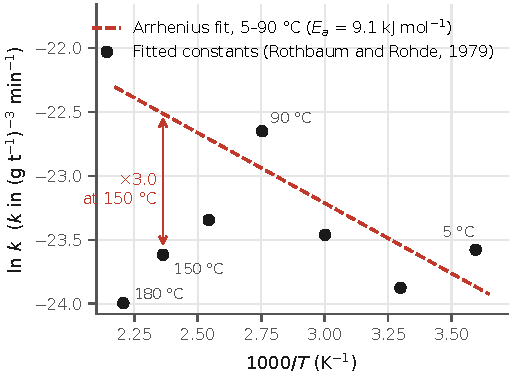
\includegraphics[width=.62\linewidth]{Figure_1}
\caption{Non-Arrhenius rate constant of amorphous-silica
polymerization. Fitted fourth-order rate constants $k(T)$ between 5 and
180~$^{\circ}$C from the primary data of \citet{rothbaum1979rohde}. The
dashed Arrhenius fit to the 5--90~$^{\circ}$C constants
($E_a = 9.1$~kJ/mol) overpredicts $k$ at 150~$^{\circ}$C by a factor of
3.0.}\label{fig:arrhenius}
\end{figure}

\begin{figure}[t]\centering
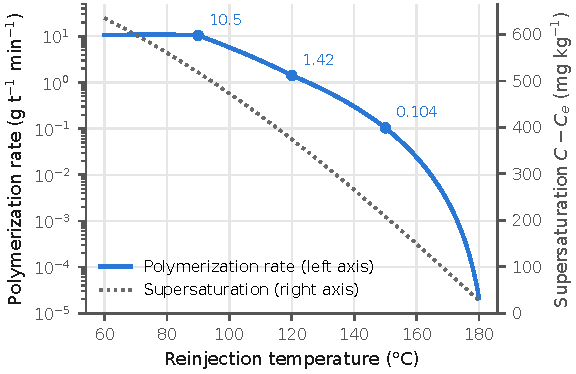
\includegraphics[width=.62\linewidth]{Figure_2}
\caption{The reinjection-temperature lever. Uninhibited polymerization
rate (left axis) and supersaturation (right axis) versus reinjection
temperature for the archetype brine: Tiwi endmember B, 638~mg/kg
reservoir silica~\citep{sugiaman2004geochemical}, at a flash fraction of
0.25 (scenario input), giving 851~mg/kg in the separated brine;
solubility from \citet{gunnarsson2000amorphous}; kinetics from the
checksum-validated transcription of \citet{rothbaum1979rohde}. Cooling
from 150 to 90~$^{\circ}$C raises the rate by a factor of
101.}\label{fig:lever}
\end{figure}

\subsection{Test against independent laboratory data}\label{sec:labtest}

The kinetic core and the solubility correlation were tested against
data to which neither was fitted: the supplementary dataset of
\citet{scott2024silica}, read with the corrected parameterization of
\citet{scott2024corrigendum}. It comprises 61 monomeric-silica decay
experiments with 1{,}275 points spanning 23--80~$^{\circ}$C, pH
2.1--10.0 and ionic strength 0.01--0.53~mol/kg. Because the source is
machine-readable, transcription gives way to automated integrity
checks: unit headers are pinned, concentrations must decay
monotonically, replicate runs listed under duplicated identifiers are
separated, and one experiment in the colloid regime, outside the
dissolved-monomer scope, is flagged.

Two properties of the kinetic core are tested separately because they
fail differently. The first is the functional form. Linearizing the
integrated $n$-th-order decay law for $n = 2, \dots, 6$ in each
experiment shows that the decay of a single curve is second order in
supersaturation: the median $R^2$ is \NUM{KvRtwo} at $n = 2$ and
\NUM{KvRfour} at $n = 4$, falls steadily as the assumed order rises, and
order 2 fits best in all \NUM{KrN} qualifying near-neutral experiments
(pH 5--8; Fig.~\ref{fig:kinval}). This does
not contradict the classical law, which correlates the maximum rate
against the initial supersaturation across separate batches; the
integrated decay of one curve follows second-order kinetics of the
Rimstidt--Barnes type~\citep{rimstidt1980kinetics}. The two describe
different observables. The second property is the rate level. The
observed second-order constants follow an Arrhenius trend with
$E_a \approx$~\NUM{KvEa}~kJ/mol, and the ratio of the observed decay constant to
the one implied by the fitted core has a median of \NUM{KrMed}, ranging
from \NUM{KrMin} to \NUM{KrMax} across the \NUM{KrN} experiments: the
modern data decay six times faster than the classical law predicts at
the median. The median sets the fast-kinetics regime of
Section~\ref{sec:design}, and the spread shows that no fixed correction
of the transcribed law would reproduce the modern data.

The plateau of a nearly complete decay experiment is an independent
measurement of amorphous-silica solubility. Sixteen near-neutral
experiments that consumed at least 70\% of their initial
supersaturation level off at 0.90--1.37 times the
\citet{gunnarsson2000amorphous} correlation, with a median of 1.05. The
correlation and the 2024 endpoints therefore agree, and the band
$[0.90, 1.37]$ is the solubility range of the sensitivity study
(Section~\ref{sec:sobol}).

\begin{figure}[t]\centering
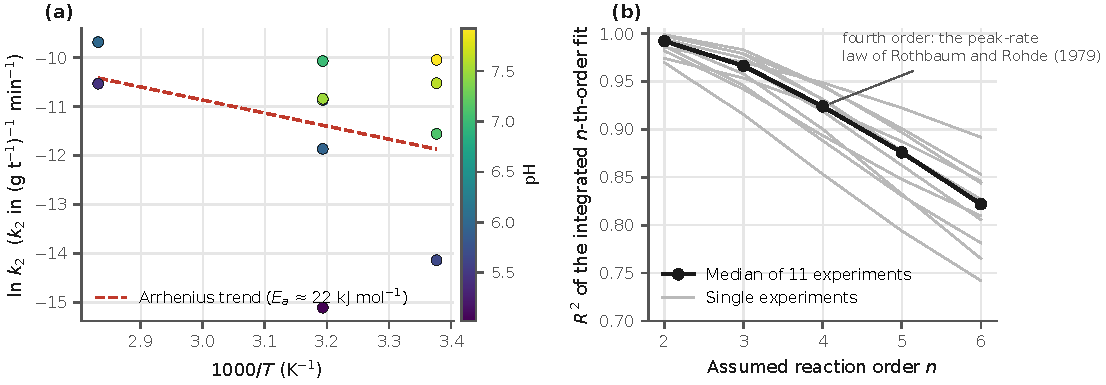
\includegraphics[width=\linewidth]{Figure_3}
\caption{Test of the kinetic core against the independent data of
\citet{scott2024silica}. (a) Observed second-order rate constants of the
\NUM{KrN} near-neutral experiments (pH 5--8) versus inverse temperature,
coloured by pH, with the Arrhenius trend. (b) $R^2$ of the integrated
$n$-th-order linearization in each experiment (grey) and the median
(black): single-curve decay is second order, while the fourth-order
form of the classical law is a peak-rate law. Source:
\texttt{results/kinetics\_validation.csv}; panel (b) recomputed within
the same fitting window.}
\label{fig:kinval}
\end{figure}

\section{Simulated line, soft sensor and optimizer}\label{sec:methods}

\subsection{Simulated brine line}\label{sec:plant}

An estimator or an optimizer tested against a plant that behaves
exactly as its model assumes proves little. The simulated line
therefore uses the kinetics of Section~\ref{sec:kinetics} with
structured deviations, each parameterized and documented. The true
polymerization rate is
\begin{equation}\label{eq:truth}
r_{\mathrm{true}} \;=\; f_u(u)\, e^{B(T)}\, k(T)\, s^{\,n},
\qquad s = C - C_e(T)\,\beta_e ,
\end{equation}
gated by an induction clock. Here $k(T)$ and $C_e(T)$ are the
literature-fitted rate constant and solubility; $B(T)$ is a smooth
log-normal bias drawn per plant on the seven kinetic isotherm nodes
($\sigma = 0.35$); the reaction order is drawn as
$n \sim \mathcal{N}(4, 0.15)$ and clipped to $[3.6, 4.4]$, in keeping
with the ``approximately fourth order'' of the source data;
$\beta_e \sim \mathcal{N}(1, 0.03)$ perturbs the solubility; and $f_u$
is a per-plant instance of the non-monotonic dose--response family of
Section~\ref{sec:kinetics}, with the maximum suppression drawn about
0.50 (standard deviation 0.10), the dose of maximum effect drawn
log-normally about 1~ppm (log standard deviation 0.25), and a mild
reversal on overdose. The induction period is fitted from the primary
kinetic dataset, $\log_{10} P = a + b \log_{10} s + cT$ with
$b = -4.31$ and $r^2 = 0.88$, a relation that reproduces the source
publication's own graphical correlation. The plant keeps a
supersaturation-exposure clock that the model lacks.

The mixture weights of the four endmembers follow a mean-reverting
Ornstein--Uhlenbeck process about the operating composition, and the
flash fraction fluctuates within $[0.20, 0.30]$, so that the separated
brine wanders inside the flashed envelope while remaining stationary
(a drift of about 1.3\% over ten days). An earlier random-walk form,
which drifted toward the mixture centroid and diluted the brine over
time, was replaced, and stationarity is now one of the repository's
automated checks.

The measurement layer follows what a shift-based operation provides:
silica grab samples every 8~h at 5\% relative noise, a continuous line
temperature with $\sigma = 0.3$~$^{\circ}$C, and one daily measurement
of the trailing-24-h mean polymerization rate at 10\% relative noise.
The rate measurement stands for a daily polymerization test, in which
the decline of monomeric silica in a brine sample is followed at line
conditions as in field inhibitor trials~\citep{baltazar2014grc}, or for
an online scale sensor~\citep{okazaki2017fiber}. A fourteen-day episode
thus provides 42 concentration samples and 14 rate labels against
2{,}016 hidden values of the true rate. A step-wise interface reproduces
the batch simulator's trajectory to machine precision, so that in
closed loop the optimizer decides each day from what it has observed.

\subsection{Hybrid soft sensor}\label{sec:sensor}

The sensed quantity is the trailing-24-h mean polymerization rate, the
quantity that accumulates scale and the one the optimizer constrains.
The sensor is a parallel hybrid~\citep{thompson1994modeling,%
vonstosch2014hybrid},
\begin{equation}\label{eq:sensor}
\hat r \;=\; \max\!\Big[\,0,\;
\exp\!\big(\log(1{+}r_{\mathrm{core}}) + \lambda\, g_{\theta}(x)\big) - 1
\Big],
\end{equation}
in which $r_{\mathrm{core}}$ is the trailing mean of the kinetic core
combined with the nominal dose--response, and $g_{\theta}$ is a
gradient-boosted residual~\citep{ke2017lightgbm} in $\log(1{+}\cdot)$
space over causal trailing-window aggregates of the measurements only;
a code-level guard raises an error if any hidden plant variable reaches
the feature set. Each sensor is trained on its own plant's sparse daily
labels under strict temporal splits, the standard soft-sensor
protocol~\citep{kadlec2009data}.

The protocol matters. Asked to generalize zero-shot to unseen plant
realizations, the residual lost to both a pure-physics and a pure-data
baseline. The reason is structural: per-plant mismatch cannot be
predicted before any data from that plant exist, whereas a sensor
trained on its plant's history and predicting forward in time can
identify that plant's bias. Two protective mechanisms follow. The
residual weight $\lambda$ in Eq.~\eqref{eq:sensor} is set by
leave-one-out (LOO) credibility on the training labels,
\begin{equation}\label{eq:lambda}
\lambda^{\ast} = \min\!\Big(1,\, \max\!\Big(0,\,
\frac{\langle e, \tilde r\rangle}{\langle \tilde r, \tilde r\rangle}\Big)\Big),
\quad \text{with } \lambda = 0 \text{ unless the LOO SSE improves by at least } 15\%,
\end{equation}
where $e$ collects the residual targets and $\tilde r$ their LOO
predictions, so that the correction is used only to the extent that it
has shown out-of-sample signal and the sensor falls back to its physics
prior when labels are few or uninformative. The same LOO computation
gives the residual's prediction-error standard deviation
$\sigma_{\mathrm{LOO}}$, which the optimizer can use as the sensor's
own statement of uncertainty.

\subsection{Daily optimization of temperature and dose}\label{sec:rto}

The decision variables are the reinjection temperature set-point and
the inhibitor dose, $(T_r, u)$, refreshed once a day following the
two-layer structure of steady-state real-time
optimization~\citep{darby2011rto}. The objective is the revenue of the
power in Eq.~\eqref{eq:power} minus the inhibitor cost. The scaling
constraint is enforced on every vertex of the brine envelope at the
adverse flash bound,
\begin{equation}\label{eq:rto}
\max_{T_r,\,u}\; J(T_r, u)
\quad \text{s.t.} \quad
r_v(T_r, u) \;\le\; r_{\max} \quad \forall v \in \mathcal{V},
\end{equation}
where $r_v = k(T_r)\,(C_v - C_e(T_r))^4 f(u)$ is the kinetic core at
the silica concentration $C_v$ of vertex $v$, $f$ is the nominal
dose--response, and $r_{\max} = 0.5$~g\,t$^{-1}$\,min$^{-1}$
(Section~\ref{sec:units} relates it to wall growth). The problem is
solved by dense grid search over 95--175~$^{\circ}$C and 0--4~ppm
($161 \times 81$ points, steps of 0.5~K and 0.05~ppm): on a bounded
two-dimensional decision space the grid is global, deterministic and
auditable, and its vectorized form is checked against the reference
solver at start-up. Solved once and held, Eq.~\eqref{eq:rto} is the
open-loop robust policy.

\subsection{Feedback corrections compared}\label{sec:feedback}

Once a day the plant returns one noisy label $\ell_t$ of the
trailing-24-h mean rate. Three ways of using it are compared, all of
which correct the constraint of Eq.~\eqref{eq:rto} and leave the
objective unchanged. The gradient corrections of full modifier
adaptation~\citep{marchetti2009modifier,marchetti2010dual} are not
attempted, because one noisy label per day does not support estimating
plant gradients.

\subsubsection{Scalar correction and its anchor}\label{sec:anchor}

The zeroth-order scheme of \citet{chachuat2008constraint} filters the
constraint bias,
\begin{equation}\label{eq:ca}
\varepsilon_t = (1-\alpha)\,\varepsilon_{t-1}
 + \alpha\,\big(\ell_t - r_a(T_{r,t}, u_t)\big)
\quad \text{and} \quad
r_v + \varepsilon_t \le r_{\max},
\end{equation}
with $\alpha = 0.5$. A log-space variant filters
$\ln \ell_t - \ln r_a$ and scales the constraint by $e^{\theta_t}$. The
model rate $r_a$ against which the label is compared is the
\emph{anchor} of the correction, and the results turn on it. With the
\emph{design-case anchor}, $r_a = r_B$: the kinetic core at the
composition the optimizer is solved against, the envelope vertex
nearest the operating brine at the adverse flash bound. With the
\emph{measured anchor}, $r_a = k(T_r)\,(C_m - C_e(T_r))^4 f(u)$: the
core at the latest silica grab sample $C_m$.

\subsubsection{Gaussian-process residual}\label{sec:gp}

The constraint model becomes $\log(1+\hat r_v) = \log(1+r_v) + \mu(x)$,
where $\mu$ is the posterior mean of a Gaussian process trained on the
residual targets $\log(1+\ell_t) - \log(1+r_a)$ at the measured anchor,
with inputs $x = (T_r, u, C_m - C_e)$, a constant mean and a
squared-exponential kernel with one length scale per input plus noise.
Hyperparameters are chosen by exact marginal likelihood over a fixed
grid, so the fit is deterministic. This arm takes from modifier
adaptation with Gaussian
processes~\citep{ferreira2018gpma,delriochanona2021tale} the idea of a
learned mismatch model that reports its own uncertainty. It does not
implement those methods' cost modifiers, acquisition functions or trust
regions, and it tests the regressor, not those algorithms.

\subsubsection{Hybrid sensor}\label{sec:hybridarm}

The trained sensor of Section~\ref{sec:sensor} is used as the
constraint model, $\log(1+\hat r_v) = \log(1+r_v) + \lambda\,
g_\theta(x)$, queried at steady state across the decision grid. Its
residual target and anchor are those of the Gaussian-process arm. The
two differ in the regressor and in the inputs: the hybrid receives the
sensor's full set of trailing-window features, the Gaussian process the
three listed above.

\subsubsection{Uncertainty back-off}\label{sec:backoff}

Each correction can be backed off by a gain $\kappa$ times its own
uncertainty estimate,
\begin{equation}\label{eq:backoff}
\text{scalar: } r_v + \varepsilon_t + \kappa\,\sigma_u \le r_{\max},
\qquad
\text{learned: } \log(1+\hat r_v) + \kappa\,\sigma \le \log(1+r_{\max}),
\end{equation}
where $\sigma_u$ is the standard deviation of the scalar scheme's
one-step prediction error over the trailing 14 days, and $\sigma$ is the
Gaussian-process predictive standard deviation or the hybrid's
$\sigma_{\mathrm{LOO}}$. The gain is swept over
$\kappa \in \{0, 0.5, 1, 2\}$. The three uncertainty estimates have
different scales, so equal $\kappa$ does not mean equal caution, and the
families are compared as curves over the sweep, not gain by gain. The
learned models are refitted weekly once seven labels exist. Until then
they run the measured-anchored scalar correction restricted to
tightening ($\varepsilon \ge 0$), so that feedback cannot relax the
constraint before a model has earned credibility.

\subsection{Simulation experiments}\label{sec:design}

The estimation experiment simulates \NUM{T1plants} plant realizations
for 90 days each; sensors are trained on the labels of the first 60
days and tested on the final 30.

The closed-loop experiment runs every policy on \NUM{CLplantsB} plant
realizations for \NUM{CLdays} days in each of two regimes. The
\emph{benign} regime uses the random per-plant deviations of
Section~\ref{sec:plant}. The \emph{stress} regime is a single-factor
perturbation: the plant's true rate is six times the model's, with all
random draws set to zero. Its size is measured, not chosen; it is the
median gap of Section~\ref{sec:labtest}. A violation day is a day whose
realized trailing-24-h mean rate exceeds $r_{\max}$. Violations are
counted on the realized plant, not on the worst-case vertex of the
envelope, from day 2 and, after the 8-day warm-up of the learned models,
from day 9. Power gains are relative to fixed practice. Every policy
meets the same brine and mismatch realization on a given plant, so
policies are compared by paired differences over plants, with seeded
percentile-bootstrap 95\% intervals (4{,}000 resamples, plants as the
resampling unit).

Two kinds of evidence are kept apart. On six of the twenty plants per
regime, the hybrid arm at $\kappa \in \{0, 1\}$ and the open-loop
policy formed a protocol whose pass criteria were fixed before it was
run; its verdicts are reported as registered in
Section~\ref{sec:models}. Everything else in
Sections~\ref{sec:anchoring} to~\ref{sec:operating}, namely the
anchoring ablation, the scalar and Gaussian-process families, the gain
sweep and the fourteen further plants, was added afterwards with
earlier results in view, and is post hoc.

\section{Results}\label{sec:results}

\subsection{Estimating the scaling rate from sparse labels}\label{sec:estimation}

Table~\ref{tab:ablation} compares the hybrid sensor with its kinetic
core and with a purely data-driven model on the unseen test windows.
\begin{table}[t]\centering
\caption{Estimation on unseen test windows: RMSE in
$\log(1{+}\cdot)$ rate space (mean $\pm$ sd over \NUM{T1plants} plant
realizations) and the fraction of estimates within a factor of two of
the hidden truth. Generated from
\texttt{results/table1\_summary.csv}.}
\label{tab:ablation}
\begin{tabular}{lccc}
\toprule
Estimator & RMSE$_{\log 1p}$ & vs.\ physics & within $\times 2$ \\
\midrule
% GENERATED by manuscript/make_numbers.py — do not edit
Physics core & $0.346 \pm 0.181$ & --- & 41\% \\
Pure ML & $0.258 \pm 0.069$ & $-25\%$ & 64\% \\
Hybrid & $0.170 \pm 0.037$ & $-51\%$ & 84\% \\

\bottomrule
\end{tabular}
\end{table}
The hybrid reduces error by \NUM{T1redPh}\% against its physics prior
and by \NUM{T1redMl}\% against the data-driven model, and it places
\NUM{T1Hywf}\% of its estimates within a factor of two of the hidden
truth, against \NUM{T1Phwf}\% and \NUM{T1Mlwf}\%. Fig.~\ref{fig:scarcity}
shows how few labels this takes. With \NUM{ScDayMin} days of labels the
hybrid (\NUM{ScHyMin}) already outperforms the physics core given any
amount of data (at best \NUM{ScPhBest}) and the data-driven model given
all \NUM{ScDayMax} days (\NUM{ScMlMax}). A transfer test bounds the
claim: a residual carried to another plant together with its donor's
credibility does harm (\NUM{TrHy} against \NUM{TrPh} for the physics
prior, mean over \NUM{TrPlants} unseen plants), which is why $\lambda$
must be earned from the target plant's own labels. With no labels,
$\lambda = 0$ and the sensor is its prior.

\begin{figure}[t]\centering
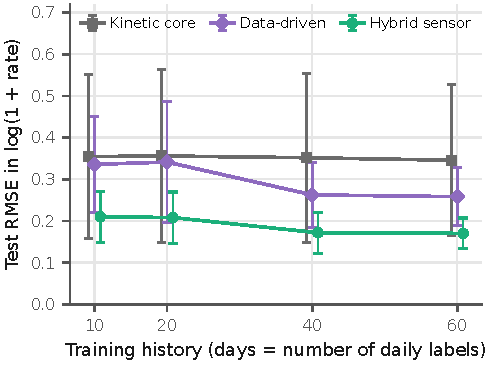
\includegraphics[width=.62\linewidth]{Figure_4}
\caption{Estimation error versus the number of daily labels. Test RMSE
in $\log(1{+}\text{rate})$ of the kinetic core, the data-driven model and
the hybrid sensor; mean $\pm$ sd over \NUM{T1plants} plant realizations,
with points offset horizontally for legibility. Generated from
\texttt{results/scarcity\_sweep.csv}.}\label{fig:scarcity}
\end{figure}

The same correction pattern was replayed on laboratory truth
(Fig.~\ref{fig:sensorval}). Each of the \NUM{SvN} decay experiments of
\citet{scott2024silica} at pH 5--8 that consumed at least half of its
supersaturation and yields at least six usable rate intervals is treated
as a plant, with interval-average observed rates as the hidden truth,
the fitted core as the prior and only the first $K$ intervals as labels.
Three corrections with honestly counted parameters are compared: none,
that is the core alone; a one-parameter offset in log space, which can
be fitted from a single label where a data-only model cannot operate at
all; and a two-parameter affine correction whose slope in $\ln s$ is, by
construction, a correction of the reaction order. Second-order truth
against a fourth-order core predicts a slope $b \approx -2$. Fitted
without restraint, the affine correction fails: early labels span almost
no supersaturation (a spread in $\ln s$ of 0.047 against 2.61 over the
test window), the fitted slopes range from \NUM{SvAffMin} to
\NUM{SvAffMax}, and the correction does far worse than none. Under the
same credibility rule as the field sensor, a leave-one-out choice
between the offset and a clipped affine correction, the method keeps
the offset until the labels support a slope ($K \le 3$), and with one
to three labels the offset is level with the core (median RMSE
\NUM{SvOffLo}--\NUM{SvOffHi} against \NUM{SvPhysLo}--\NUM{SvPhysHi}). At
$K = 5$ the slope is adopted in \NUM{SvSelfive} of the \NUM{SvNfive}
experiments long enough to be scored, with a median $b =$~\NUM{SvBfive}
that independently recovers the second-order finding, and the
correction wins with a median RMSE of \NUM{SvCredfive} against
\NUM{SvPhysfive} for the core. The lesson carries over to the plant: a
correction should have no more freedom than the labels can identify,
and a line held near one operating point presents a level-dominated
problem in which a scalar correction is well identified.

\begin{figure}[t]\centering
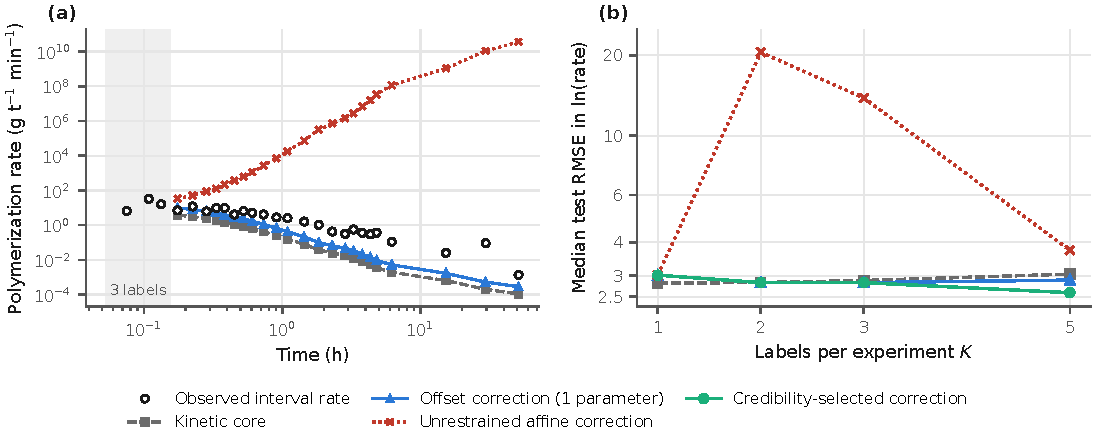
\includegraphics[width=\linewidth]{Figure_5}
\caption{The correction pattern on laboratory decay curves.
(a) Experiment \NUM{SvExp} of \citet{scott2024silica}
(\NUM{SvExpT}~$^{\circ}$C, pH \NUM{SvExpPH}) with three labels (shaded):
observed interval rates, the kinetic core, the one-parameter offset
correction, which with three labels is also the credibility-selected
correction, and the unrestrained affine correction, which diverges.
(b) Median test RMSE over the \NUM{SvN} experiments (\NUM{SvNfive} at
$K = 5$) versus the number of labels $K$. Source:
\texttt{results/sensor\_validation\_scott.csv}.}
\label{fig:sensorval}
\end{figure}

\subsection{The anchor of the correction decides safety}\label{sec:anchoring}

Table~\ref{tab:closedloop} gives the closed-loop results for fixed
practice, the open-loop robust policy and the scalar corrections, and
Fig.~\ref{fig:frontier} shows every policy as a trade-off between power
gain and violations; Table~S1 of the Supplementary material lists the
Gaussian-process and hybrid corrections in the same format.

\begin{table}[!tbp]\centering\footnotesize
\setlength{\tabcolsep}{3.2pt}\renewcommand{\arraystretch}{0.78}
\caption{Closed-loop results, mean over \NUM{CLplantsB} plant
realizations $\times$ \NUM{CLdays} days per regime. Gain is gross power
over fixed practice (mean $\pm$ sd over plants, \%). Violation days are
means per run with the worst plant in parentheses; ``post-w.'' counts
days after the 8-day warm-up. The scalar correction computed at the
measured silica without back-off is the $\kappa = 0$ row of the last
block. Generated from \texttt{results/table2\_summary.csv} and
\texttt{results/table2b\_summary.csv}.}
\label{tab:closedloop}
\begin{tabular}{lccccc}
\toprule
 & \multicolumn{2}{c}{Benign regime} & \multicolumn{3}{c}{Stress regime
 ($\times 6$)} \\
\cmidrule(lr){2-3}\cmidrule(lr){4-6}
Policy & Gain & Viol.\ days & Gain & Viol.\ days & Post-w. \\
\midrule
% GENERATED by manuscript/make_numbers.py — do not edit
Fixed practice & --- & 0.00 (0) & --- & 0.00 (0) & 0.00 \\
Robust optimum, no feedback & $+41.7 \pm 0.0$ & 0.45 (7) & $+41.7 \pm 0.0$ & 20.65 (28) & 17.50 \\
\addlinespace
\multicolumn{6}{l}{\emph{Anchoring ablation: scalar correction computed at}} \\
\quad design case, additive & $+81.5 \pm 20.7$ & 5.60 (17) & $+37.3 \pm 2.5$ & 15.80 (18) & 13.25 \\
\quad design case, log-space & $+100.3 \pm 33.5$ & 17.80 (21) & $+41.3 \pm 3.2$ & 19.20 (26) & 16.35 \\
\quad measured silica, log-space & $+3.4 \pm 52.2$ & 0.35 (2) & $-46.7 \pm 15.7$ & 0.25 (1) & 0.15 \\
\addlinespace
\multicolumn{6}{l}{\emph{Scalar correction at measured silica, back-off gain $\kappa$}} \\
\quad $\kappa = 0$ & $+40.6 \pm 7.1$ & 0.00 (0) & $+21.1 \pm 1.5$ & 1.60 (6) & 1.25 \\
\quad $\kappa = 0.5$ & $+34.8 \pm 6.1$ & 0.00 (0) & $+15.9 \pm 2.0$ & 0.65 (2) & 0.45 \\
\quad $\kappa = 1$ & $+29.3 \pm 5.6$ & 0.00 (0) & $+10.6 \pm 2.6$ & 0.40 (1) & 0.20 \\
\quad $\kappa = 2$ & $+18.6 \pm 6.6$ & 0.00 (0) & $-1.1 \pm 4.5$ & 0.25 (1) & 0.05 \\

\bottomrule
\end{tabular}
\end{table}

\begin{figure}[!tbp]\centering
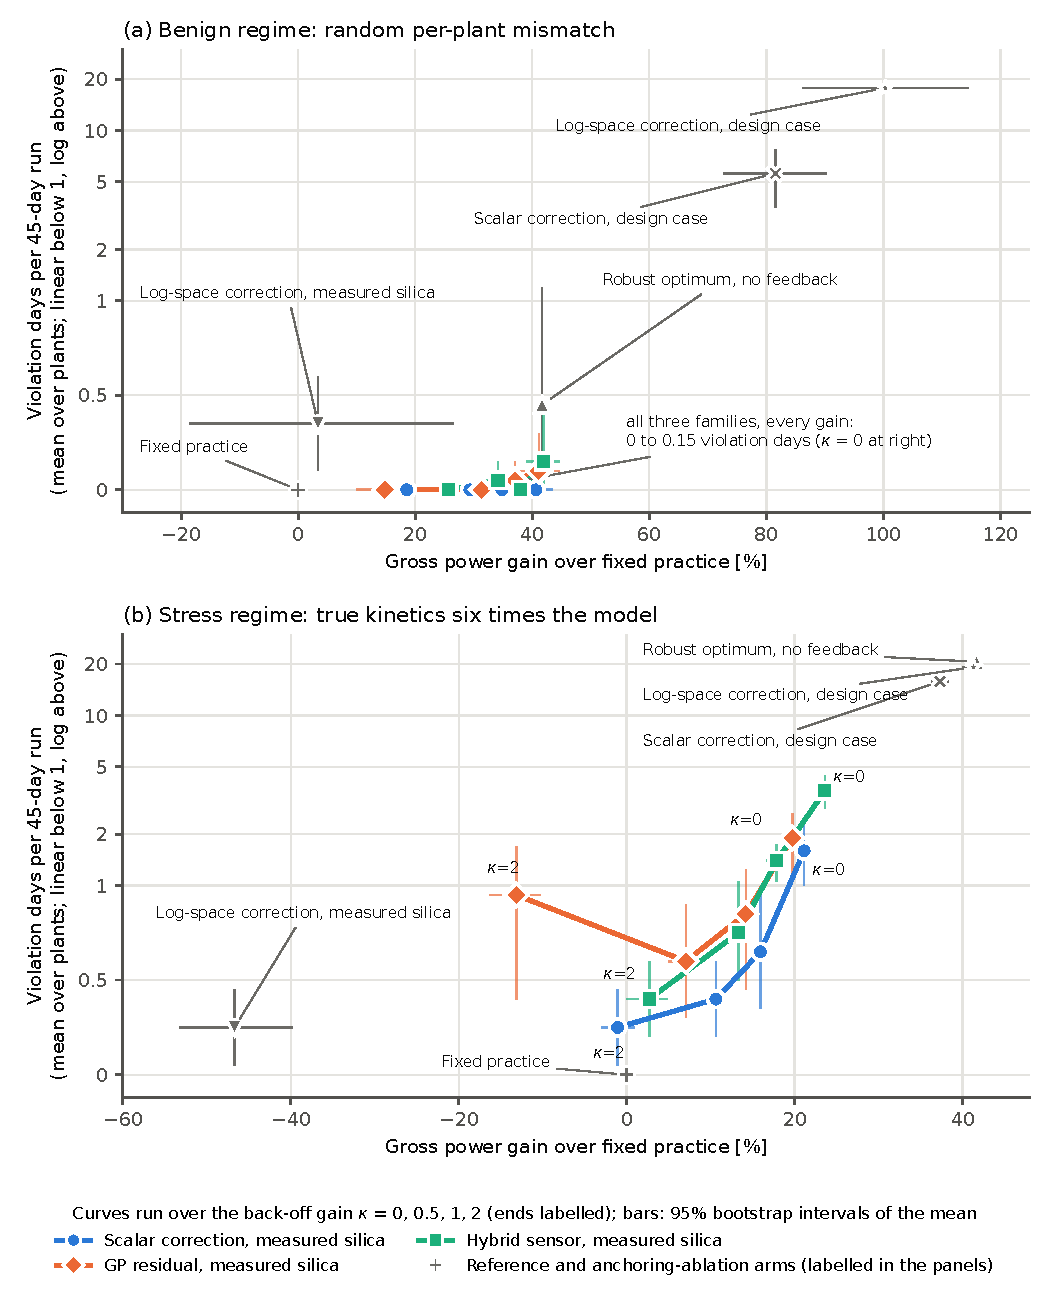
\includegraphics[width=\linewidth]{Figure_6}
\caption{Trade-off between power gain and safety for every policy. Each
correction computed at the measured silica is a curve over the back-off
gain $\kappa = 0, 0.5, 1, 2$, with $\kappa = 0$ at the high-gain end;
fixed practice, the open-loop policy and the anchoring-ablation arms are
single labelled markers. Bars are 95\% bootstrap intervals of the mean
over plants. The vertical axis is linear below one violation day and
logarithmic above. Generated from
\texttt{results/closed\_loop\_frontier.csv}.}\label{fig:frontier}
\end{figure}

Consider the anchoring block of Table~\ref{tab:closedloop}. Computed at
the design case, the additive correction averages \CL{B}{CAnom}{v}
violation days per run in the benign regime (\CL{B}{CAnom}{m} on the
worst plant) and \CL{S}{CAnom}{v} in the stress regime, against
\CL{S}{Open}{v} with no feedback at all. Computed at the measured silica
concentration, the same correction at the same gain averages
\CL{B}{CAk0}{v} and \CL{S}{CAk0}{v}. The paired reductions are
\CT{anchorB}{v}{abs} days (95\% interval
\CT{anchorB}{v}{lop}--\CT{anchorB}{v}{hip}) and \CT{anchorS}{v}{abs}
days (\CT{anchorS}{v}{lop}--\CT{anchorS}{v}{hip}). The log-space
correction behaves the same way under stress, with \CL{S}{LGnom}{v}
against \CL{S}{LGmeas}{v} violation days.

A diagnostic isolates the mechanism. With the operating point held at
the open-loop optimum on the \NUM{AnPlants} stress plants, the model
error that a correction ought to see is a constant factor of six, and
the ratio of each day's label to the anchor model can be formed
directly. The design-case brine is more concentrated than the brine the
plant actually carries, so through the fourth-power rate law the
design-case model over-predicts the realized-brine model by a median
factor of \NUM{AnMarginmed}. That factor is the safety margin of the
robust optimizer. A correction computed at the design case sees the
product of this margin and the model error and cannot separate them.
Under the sixfold stress the two nearly cancel: the ratio of label to
design-case model has a median of \NUM{AnDesmed} (5th to 95th
percentile \NUM{AnDeslo}--\NUM{AnDeshi}), the correction finds almost
nothing to correct, and the line is left where the realized rate
exceeds the limit on \NUM{AnShare}\% of days. In the benign regime,
with no systematic kinetic error, the same correction reads the margin
as excess caution, relaxes the constraint, cools the line and violates.
Computed at the measured silica, the ratio has a median of
\NUM{AnMeasmed}, close to the kinetic error it should see.

That margin and stress are of nearly equal size here is a coincidence;
the confounding is not. Any scheme that is solved against a worst-case
envelope and corrected from plant feedback must compare the feedback
with the model at the realized conditions, or it will mistake its own
safety margin for model error, in whichever direction the two happen to
combine.

The diagnostic also explains why the log-space correction is so
cautious at the measured anchor. The measured-anchor ratio is
heavy-tailed (95th percentile \NUM{AnMeashi}) because on some days the
measured supersaturation is small and the model rate nearly vanishes.
An additive correction is insensitive to that tail, since a small model
rate yields a small absolute innovation; a multiplicative correction is
not, and under stress it ran the line hotter than fixed practice
(\CL{S}{LGmeas}{u}\% power).

\subsection{Correction model and back-off}\label{sec:models}

In the benign regime, once computed at the measured silica, all three
corrections are essentially free of violations. Without back-off the
scalar correction has no violation day on any of the \NUM{CLplantsB}
plants, the Gaussian-process residual averages \CL{B}{GPk0}{v} and the
hybrid \CL{B}{HYk0}{v}, at power gains of \CL{B}{CAk0}{u}\%,
\CL{B}{GPk0}{u}\% and \CL{B}{HYk0}{u}\%. These gains are those of the
open-loop robust policy (\CL{B}{Open}{u}\%), which nevertheless violates
on \CL{B}{Open}{v} days on average and \CL{B}{Open}{m} on its worst
plant, because an envelope over brine chemistry does not protect
against kinetic deviations. Here feedback buys safety rather than
power, and back-off costs power while buying nothing: $\kappa = 1$
takes \NUM{boCAB} points off the scalar correction's gain with no change
in violations.

In the stress regime the open-loop policy violates on \CL{S}{Open}{v}
days per run, and the three corrections separate into the curves of
Fig.~\ref{fig:frontier}(b). Without back-off the scalar correction keeps
a gain of \CL{S}{CAk0}{u}\% at \CL{S}{CAk0}{v} violation days. The
hybrid gains slightly more (\CL{S}{HYk0}{u}\%) and violates more
(\CL{S}{HYk0}{v} days; paired difference \CT{HYk0S}{v}{d}, interval
\CT{HYk0S}{v}{lop} to \CT{HYk0S}{v}{hip}). The Gaussian process gains
slightly less (\CL{S}{GPk0}{u}\%) at a violation count
indistinguishable from the scalar's (difference \CT{GPk0S}{v}{d},
interval \CT{GPk0S}{v}{lop} to \CT{GPk0S}{v}{hip}). Back-off moves each
family along its curve at a similar price. From $\kappa = 0$ to
$\kappa = 1$ the scalar correction gives up \CT{boCA}{u}{abs} points of
gain and \CT{boCA}{v}{abs} violation days, the hybrid
\CT{boHY}{u}{abs} points and \CT{boHY}{v}{abs} days, and the Gaussian
process \CT{boGP}{u}{abs} points and \CT{boGP}{v}{abs} days. At
$\kappa = 2$ the scalar and hybrid corrections are down to
\CL{S}{CAk2}{w} and \CL{S}{HYk2}{w} post-warm-up violation days, with
almost no gain left (\CL{S}{CAk2}{u}\% and \CL{S}{HYk2}{u}\%). Under a
sixfold kinetic error there is little extra power that is safe to take.

Read as curves, the families overlap, and no learned model dominates
the scalar correction. At equal gain the hybrid sits a few points of
power to the right of the scalar curve and somewhat above it (at
$\kappa = 1$: \CT{HYk1S}{u}{d} points, \CT{HYk1S}{v}{d} violation days),
which is a different point on a similar curve rather than a better
curve. The Gaussian-process family lies slightly inside the scalar one,
with less gain at every $\kappa$ and, at $\kappa = 2$, more violations
as well (\CT{GPk2S}{u}{d} points, \CT{GPk2S}{v}{d} days). A plausible
reason is that a wide posterior away from the visited operating points
pushes the optimizer into regions the model has not seen, the failure
that trust regions address in the Gaussian-process
literature~\citep{delriochanona2021tale}. Two further explanations are
offered, neither of which the experiments isolate. A line held near one
operating point needs a correction that is local and current, which a
scalar updated daily supplies and models refitted weekly do not. And
the hybrid's credibility shrinkage pulls its correction toward a
kinetic prior that, under stress, under-predicts sixfold; that protects
estimation accuracy but is the unsafe direction for control, and
without back-off the hybrid has the most violations of the three.

On the six plants of the registered protocol, the open-loop policy
violates chronically (\NUM{PreOpenv} days), as expected. The hybrid
without back-off averages \NUM{PreHYk0w} post-warm-up violation days,
missing its registered target of zero. The hybrid with $\kappa = 1$
averages \NUM{PreHYk1w} days against a registered criterion of at most
0.5, and it is safer than the arm without back-off, as registered. These
figures use the measured-anchored warm-up; with the original
design-case warm-up the two arms gave 2.17 and 0.50 days, and the
verdicts were the same.

\subsection{Operating points at the reinjection line}\label{sec:operating}

In plant terms the policies differ mainly in the reinjection
temperature they hold. Because gross power is linear in the temperature
drop (Eq.~\eqref{eq:power}), each plant's mean power gives its mean
reinjection temperature exactly, and its inhibitor cost gives its mean
dose. Fixed practice holds 150~$^{\circ}$C and 1~ppm. The open-loop
robust policy settles at \CL{B}{Open}{T}~$^{\circ}$C and
\CL{B}{Open}{dose}~ppm: lowering the line by \NUM{dTOpen}~K releases
\NUM{QthOpen}~MW of heat from the \NUM{Mflow}~kg/s stream, which the
assumed conversion effectiveness of \NUM{EtaB} turns into
\NUM{dMWOpen}~MW of additional gross power (\CL{B}{Open}{mw} against
\CL{B}{Fixed}{mw}~MW). In the benign regime the measured-silica
correction holds nearly the same point (\CL{B}{CAk0}{T}~$^{\circ}$C)
while removing the open-loop policy's violations, whereas the
design-case corrections cool the line to \CL{B}{CAnom}{T}~$^{\circ}$C
(additive) and \CL{B}{LGnom}{T}~$^{\circ}$C (log-space), which is where
their violations come from. In the stress regime the measured-silica
correction warms the line to \CL{S}{CAk0}{T}~$^{\circ}$C without
back-off and to \CL{S}{CAk1}{T}~$^{\circ}$C with $\kappa = 1$, while the
design-case correction stays at \CL{S}{CAnom}{T}~$^{\circ}$C, close to
the open-loop set-point. The safe response to sixfold faster kinetics
is a rise of \NUM{dTsafeA} to \NUM{dTsafeB}~K in reinjection
temperature, and the design-case correction does not find it.

The dose moves much less than the temperature. Across all optimized
policies and both regimes the mean dose lies between \NUM{DoseMin} and
\NUM{DoseMax}~ppm, below the 1~ppm of fixed practice, because the
inhibitor's suppression is flat near its optimum while its cost rises
linearly with dose. Inhibitor intensity falls from
\CL{B}{Fixed}{i}~PHP/MWh under fixed practice to \CL{B}{CAk0}{i}~PHP/MWh
under the measured-silica correction, partly through the lower dose and
mostly through the larger output over which the dose is spread.

\subsection{Sensitivity to kinetics, solubility, inhibitor response and
economics}\label{sec:sobol}

A Sobol study ($N = \NUM{SobN}$, seeded, \NUM{SobEvals} evaluations)
spans the declared uncertainty set of the open-loop optimum: a kinetic
band equal to the measured sixfold gap, the measured solubility band
$[0.90, 1.37]$, and scenario bands for the flash fraction (0.20--0.30),
the inhibitor response (maximum suppression 0.30--0.70, dose of maximum
effect 0.5--2.0~ppm), the scaling limit $r_{\max}$
(0.25--1.0~g\,t$^{-1}$\,min$^{-1}$), the conversion effectiveness
(0.08--0.14) and the electricity price (PHP~4--7/kWh)
(Fig.~\ref{fig:sobol}). Kinetic uncertainty dominates the open-loop
optimum, with total-order indices of \NUM{SobSTMw}, \NUM{SobSTT} and
\NUM{SobSTNet} on gross power, optimal temperature and net objective,
followed by solubility (\NUM{SobSTTce} on the optimal temperature). The
inhibitor response decides the dose and barely touches the temperature:
the dose of maximum effect has a total-order index of \NUM{SobSTDose}
on the optimal dose and \NUM{SobSTTdopt} on the optimal temperature,
and the maximum suppression has \NUM{SobSTTeta} on the optimal
temperature. Within the declared band, then, the assumed dose--response
family moves the dose that is chosen, not the reinjection temperature
or the power, and the benign regime already perturbs that response on
every plant (Section~\ref{sec:plant}). Feasibility holds at
\NUM{SobFeas}\% across the set. The gross-power optimum spans
\NUM{Sobmwq05}/\NUM{Sobmwq50}/\NUM{Sobmwq95}~MW
($q_{05}/q_{50}/q_{95}$); its median exceeds the nominal
\CL{B}{Open}{mw}~MW because several bands are not centred on the
nominal values and the study samples the flash fraction instead of
holding its adverse bound.

Re-valuing the closed-loop trajectories over the economic envelope
attaches ranges to every peso figure. The assumption that makes this
valid was checked rather than assumed: the optimum moves zero grid
steps across the eight corners of the envelope, with inhibitor cost
below 15\% of revenue everywhere, so power gains and violation counts
do not depend on the economic assumptions.

\begin{figure}[t]\centering
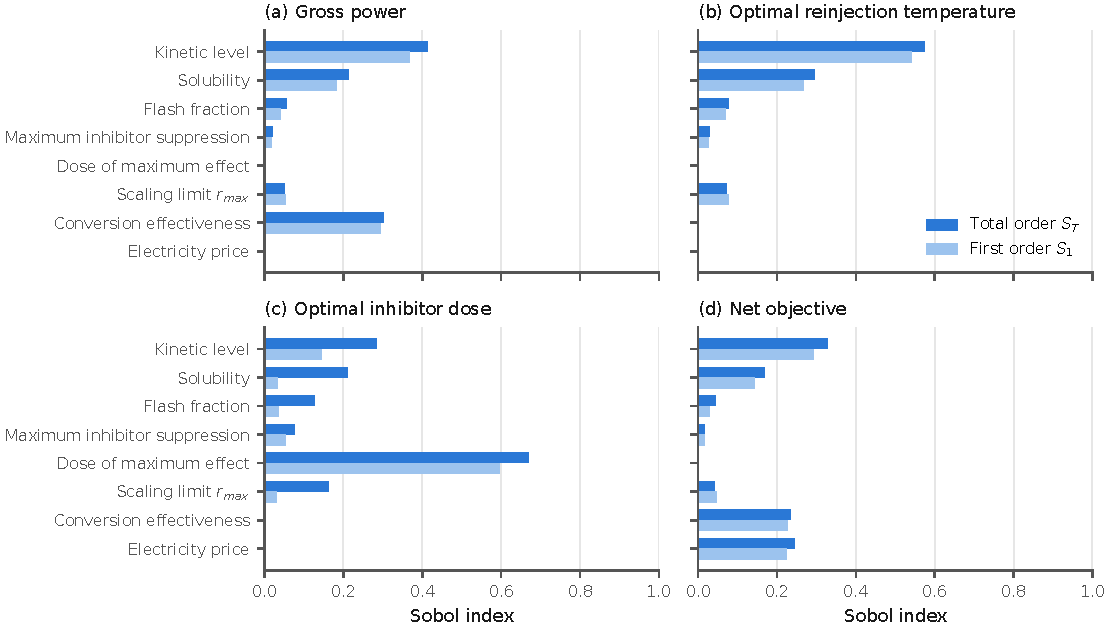
\includegraphics[width=\linewidth]{Figure_7}
\caption{Sobol sensitivity of the open-loop optimum. First-order
($S_1$) and total-order ($S_T$) indices of (a) gross power, (b) optimal
reinjection temperature, (c) optimal inhibitor dose and (d) net
objective over the declared uncertainty set. Generated from
\texttt{results/sensitivity\_sobol.csv}.}
\label{fig:sobol}
\end{figure}

\section{Discussion}\label{sec:discussion}

\subsection{Implications for field operation}\label{sec:field}

The scheme that did best is also the simplest to run. It needs the
silica grab samples that field chemistry programs already take, here
every 8~h, one scaling-rate measurement per day, and a daily calculation
that takes well under a second on a laptop. The correction is one
number per day: the measured rate minus the model rate at the measured
silica concentration and the current temperature and dose, filtered
with a gain of one half. Two choices need care. The first is the
anchor. An operator who compares the measured rate with the design-case
prediction, a natural reference when the design case is the document of
record, will read the design margin as model error. The second is the
back-off. Under sixfold faster kinetics a gain of $\kappa = 1$ on the
correction's own prediction-error standard deviation exchanged
\CT{boCA}{u}{abs} points of power gain for \CT{boCA}{v}{abs} fewer
violation days per run, while without systematic kinetic error it cost
\NUM{boCAB} points and bought nothing. A site without kinetic data of
its own should therefore start with $\kappa$ near one and lower it as
the history of the correction shows the model error to be small.
Because the safe response to a kinetic error is a few kelvin of
reinjection temperature (Section~\ref{sec:operating}), the set-point
changes the scheme asks for are of a size an operator would treat as
routine.

A field trial can reuse the pilot designs of Philippine inhibitor
programs, in which a side stream of treated brine runs through an
insulated test line with inspection spools and retention vessels while
temperature, pressure and silica are monitored~\citep{see2010wgc}. Run
at the optimized set-points, such a line would test the policy and,
through its spools, calibrate the scaling limit against wall growth.

\subsection{Scaling limit and wall growth}\label{sec:units}

The constraint is a polymerization (monomer-depletion) rate, not a rate
of wall growth. The molecular-deposition treatment of
\citet{weres1981kinetics}, transcribed under the same integrity protocol
(its printed checkpoints reproduce, including the 3.0~kcal/mol effective
activation energy; one internal inconsistency in its Eq.~[4c] is
documented and not silently repaired), converts
$r_{\max} = 0.5$~g\,t$^{-1}$\,min$^{-1}$ into a wall growth of about
0.3~mm/yr at the optimized operating point and 0.04--1.6~mm/yr across
90--175~$^{\circ}$C. That is a lower bound on scale growth. Field
deposits also grow by the aggregation and cementation of colloidal
silica~\citep{vandenheuvel2018understanding}, and inhibitor-treated
Philippine lines have shown 2.4--11.9~mm/yr in a 0.5~ppm test at Leyte
and up to about 20~mm/yr projected along a hot-injection pilot line at
Bacman~\citep{baltazar2014grc,see2010wgc}. The limit used here is
therefore a placeholder, to be calibrated against spool or coupon data
at the site. In the sensitivity study a fourfold band of $r_{\max}$
moves the optimal temperature far less than the kinetic uncertainty
does (total-order index \NUM{SobSTTrmax} against \NUM{SobSTT}).

\subsection{Limitations}\label{sec:limits}

The closed-loop results are in silico. The plant is simulated, although
every physical ingredient, from solubility and kinetics to the brine
envelope and the inhibitor response, comes from primary literature and,
wherever independent data exist, was tested against them
(Section~\ref{sec:labtest}). Component-wise validation on real data
combined with a closed loop under parameterized mismatch is an
intermediate step between simulation-only studies and a field trial,
not a substitute for the trial.

The ranking among the measured-anchored corrections holds for a line
held near one operating point, with one label per day, weekly refits of
the learned models, and the particular regressors and uncertainty
estimates used here. A line whose brine steps when wells are switched
would favour a correction that depends on the state over one that is
merely current, and that case was not tested. The Gaussian-process arm
compares a regressor, not Gaussian-process modifier adaptation, whose
trust regions and acquisition functions might change its curve.

Violations are counted on the realized plant. Every feedback policy, by
tightening or relaxing the constraint from what the plant returns,
trades the worst-case guarantee of Eq.~\eqref{eq:rto} for performance
at the realized brine. Under the sixfold stress a policy that kept the
full envelope guarantee would have to run hotter than fixed practice,
which is what the log-space correction at the measured anchor does; the
additive corrections are safe on the realized plant but would
under-correct if the brine moved to the worst-case vertex.

The chemistry is near neutral. High-pH brines need silica ionization
corrections that are deferred here (the speciation layer exists in the
repository but is not used in the loop), and acid dosing, the third
lever of Philippine practice~\citep{remoroza2008ph}, is not modeled.
Economic figures are scenario values with declared ranges.

Finally, the anchoring ablation exists because an initial analysis used
the design-case anchor for its scalar baseline and concluded, wrongly,
that the hybrid loop was the only safe policy. The ablation, the
measured-anchored scalar family, the Gaussian-process comparator, the
gain sweep and fourteen of the twenty plants were added after that
error was found. The effect of the anchor, an order of magnitude in
violation days with intervals far from zero and a mechanism reproduced
by a separate diagnostic, is secure; the finer comparisons among the
corrections were not registered in advance and would merit replication.

\subsection{Beyond silica}\label{sec:general}

The anchoring result does not depend on silica chemistry. Whenever an
operating point is optimized against a worst-case envelope of
composition and corrected from plant feedback, the feedback has to be
compared with the model at the realized composition, because at the
design case it carries the robustness margin as well as the model
error. The steeper the scaling law, the larger the margin in rate terms
and the worse the confusion: here the design-case brine, at 911~mg/kg,
is only 7\% more concentrated than the nominal operating brine, yet the
model rates at the two differ by a median factor of \NUM{AnMarginmed}. The same care applies to calcite, stibnite or barite limits set
from envelope calculations~\citep{tonkul2021characterization,%
omrani2025probabilistic}. The second lesson is more modest: on this
problem a better estimator did not make a better controller, and the
simplest correction that used the right measurement was as good as any.

\section{Conclusions}\label{sec:conclusions}

Silica scaling limits how far geothermal brine can be cooled before
reinjection, and the rate law used to set that limit differs from
independent laboratory data by a factor of \NUM{KrMed} at the median.
Under that uncertainty, and with feedback limited to silica grab
samples and one rate measurement per day, this study reached four
conclusions.
\begin{enumerate}
\item A daily correction of the scaling constraint must compare the
measured rate with the model at the measured silica concentration.
Compared with the design-case prediction, it mistakes the optimizer's
safety margin for model error: under sixfold faster kinetics the line
exceeded the scaling limit on \CL{S}{CAnom}{v} days per 45-day run,
against \CL{S}{CAk0}{v} with the measured anchor.
\item With the right anchor a scalar bias correction is enough.
Gaussian-process and gradient-boosted corrections traced overlapping
trade-offs between power and safety and did not improve on it. A
back-off of $\kappa = 1$ held violations to \CL{S}{CAk1}{v} days at a
\CL{S}{CAk1}{up}\% power gain over fixed practice under fast kinetics,
and without systematic kinetic error the correction gained
\CL{B}{CAk0}{up}\% with no violation on any plant.
\item In plant terms the safe response to fast kinetics is a few
kelvin: the corrected policy raised the mean reinjection temperature
from \CL{S}{Open}{T} to \CL{S}{CAk1}{T}~$^{\circ}$C, and the optimized
dose stayed below 1~ppm throughout.
\item A hybrid soft sensor estimates the scaling rate from sparse daily
labels with \NUM{T1redPh}\% less error than its kinetic core, provided
its correction is earned from the plant's own labels.
\end{enumerate}
The laboratory comparison also returned two findings of geochemical
interest: the decay of a single monomeric-silica curve is second order,
against the fourth-order peak-rate law, and the 2000 solubility
correlation agrees with the 2024 endpoints at a median of
$1.05\times$. A field trial on a side stream with inspection spools is
the next step.


\appendix
\section{Data transcription and integrity protocol}\label{app:protocol}
Primary numerical sources enter the repository only through a
transcription protocol: tables are transcribed to CSV against the
publisher's text layer, validated against printed derived quantities
where the source provides them (for the kinetic dataset of
\citet{rothbaum1979rohde}, the printed $R \cdot P^{1.5}$ checksum column
validates 33 of 33 retained rows; one flagged row is excluded), and
tagged with an evidence tier: T1 for peer-reviewed primary sources, T2
for conference or institutional material, and T3 for trade press, which
may motivate scenario scale only and is never fitted, a rule enforced
in code. Machine-readable sources replace manual transcription with
automated parser integrity checks (Section~\ref{sec:labtest}).

\section{Reproducibility and software development}\label{app:repro}
A single gate script executes the self-checks of all \NUM{GateModules}
modules (\NUM{GateChecks} checks at the time of writing) and refuses a
green status unless every check passes; the repository convention is
that no commit is made against a red gate. All stochastic components
are seeded, including the Sobol sampler, whose default scrambled
quasi-random sequence is pinned, and the Gaussian-process fit uses no
optimizer. The Python environment is pinned in
\texttt{requirements.txt}; principal dependencies are
NumPy/SciPy/pandas, LightGBM~\citep{ke2017lightgbm},
SALib~\citep{herman2017salib}, and PHREEQC via
phreeqpython~\citep{parkhurst2013phreeqc} for the (deferred) speciation
layer.

Two safeguards were added after the errors described in
Section~\ref{sec:limits}. Every long experiment records a digest of the
source files it depends on and of the result files it writes, and a
gate module fails when committed results no longer match the current
code, which is how a table computed before a change to the plant model
is now caught. The experimental numbers in this manuscript, including
the bodies of Tables~\ref{tab:ablation} and~\ref{tab:closedloop} and of
Table~S1, are generated from the result files by a script that also
checks each claim the text makes against the data, and are not typed.

The analysis software was developed with the assistance of a
generative AI coding assistant (Claude, Anthropic), which was used
under the author's direction to write and refactor code, to propose
automated checks and to help diagnose errors, including the baseline
error reported in this paper. The author ran the gate and all
experiments, and is responsible for the code and for the results.


% back matter after the appendices, so that the acknowledgments sit
% directly before the reference list (Geothermics guide for authors)
\section*{CRediT authorship contribution statement}
\textbf{Bien Don Busico:} Conceptualization, Methodology, Software,
Validation, Formal analysis, Investigation, Data curation,
Visualization, Writing -- original draft, Writing -- review \& editing.

\section*{Declaration of competing interest}
The author declares that he has no known competing financial interests
or personal relationships that could have appeared to influence the
work reported in this paper.

\section*{Funding}
This research did not receive any specific grant from funding agencies
in the public, commercial, or not-for-profit sectors.

\section*{Data availability}
The code, the transcribed primary data, all result files and the
scripts that regenerate every table and figure are available at\\
\url{https://github.com/beebzy-droid/e1-geothermal-silica-rto}. The
independent validation dataset is the supplementary material of
\citet{scott2024silica} and is obtained from that article; it is not
redistributed.

\section*{Declaration of generative AI and AI-assisted\\ technologies in the manuscript preparation process}
During the preparation of this work the author used Claude (Anthropic)
in order to draft and edit the text of the manuscript and to organize
its structure. After using this tool, the author reviewed and edited
the content as needed and takes full responsibility for the content of
the published article. The use of the same tool in developing the
analysis software is described in \ref{app:repro}.

\section*{Acknowledgments}
The author thanks Dr.~Samuel Scott for directing him to the study's
supplementary dataset, for clarifying the published parameterization
and its corrigendum, and for providing a reference implementation
script used for cross-checking, which is not redistributed with this
work.


\begin{thebibliography}{36}
\expandafter\ifx\csname natexlab\endcsname\relax\def\natexlab#1{#1}\fi
\providecommand{\url}[1]{\texttt{#1}}
\providecommand{\href}[2]{#2}
\providecommand{\path}[1]{#1}
\providecommand{\DOIprefix}{doi:}
\providecommand{\ArXivprefix}{arXiv:}
\providecommand{\URLprefix}{URL: }
\providecommand{\Pubmedprefix}{pmid:}
\providecommand{\doi}[1]{\href{http://dx.doi.org/#1}{\path{#1}}}
\providecommand{\Pubmed}[1]{\href{pmid:#1}{\path{#1}}}
\providecommand{\bibinfo}[2]{#2}
\ifx\xfnm\relax \def\xfnm[#1]{\unskip,\space#1}\fi
%Type = Article
\bibitem[{Baltazar et~al.(2014)Baltazar, See, {de Guzman}, Solis, Salonga,
  Ogena, Patel, Lee and Ooi}]{baltazar2014grc}
\bibinfo{author}{Baltazar, Jr., A.D.}, \bibinfo{author}{See, F.S.},
  \bibinfo{author}{{de Guzman}, R.C.}, \bibinfo{author}{Solis, R.P.},
  \bibinfo{author}{Salonga, N.D.}, \bibinfo{author}{Ogena, M.S.},
  \bibinfo{author}{Patel, S.}, \bibinfo{author}{Lee, L.}, \bibinfo{author}{Ooi,
  A.}, \bibinfo{year}{2014}.
\newblock \bibinfo{title}{Geothermal silica scale inhibition and control using
  phosphino carboxylic acid copolymer in {Bacon-Manito} geothermal business
  unit}.
\newblock \bibinfo{journal}{Geotherm. Resour. Counc. Trans.}
  \bibinfo{volume}{38}, \bibinfo{pages}{663--668}.
%Type = Article
\bibitem[{Buster et~al.(2021)Buster, Siratovich, Taverna, Rossol, Weers, Blair,
  Huggins, Siega, Mannington, Urgel, Cen, Quinao, Watt and
  Akerley}]{buster2021gooml}
\bibinfo{author}{Buster, G.}, \bibinfo{author}{Siratovich, P.},
  \bibinfo{author}{Taverna, N.}, \bibinfo{author}{Rossol, M.},
  \bibinfo{author}{Weers, J.}, \bibinfo{author}{Blair, A.},
  \bibinfo{author}{Huggins, J.}, \bibinfo{author}{Siega, C.},
  \bibinfo{author}{Mannington, W.}, \bibinfo{author}{Urgel, A.},
  \bibinfo{author}{Cen, J.}, \bibinfo{author}{Quinao, J.},
  \bibinfo{author}{Watt, R.}, \bibinfo{author}{Akerley, J.},
  \bibinfo{year}{2021}.
\newblock \bibinfo{title}{A new modeling framework for geothermal operational
  optimization with machine learning ({GOOML})}.
\newblock \bibinfo{journal}{Energies} \bibinfo{volume}{14},
  \bibinfo{pages}{6852}.
\newblock \DOIprefix\doi{10.3390/en14206852}.
%Type = Article
\bibitem[{Chachuat et~al.(2008)Chachuat, Marchetti and
  Bonvin}]{chachuat2008constraint}
\bibinfo{author}{Chachuat, B.}, \bibinfo{author}{Marchetti, A.},
  \bibinfo{author}{Bonvin, D.}, \bibinfo{year}{2008}.
\newblock \bibinfo{title}{Process optimization via constraints adaptation}.
\newblock \bibinfo{journal}{J. Process Control} \bibinfo{volume}{18},
  \bibinfo{pages}{244--257}.
\newblock \DOIprefix\doi{10.1016/j.jprocont.2007.07.001}.
%Type = Article
\bibitem[{Darby et~al.(2011)Darby, Nikolaou, Jones and
  Nicholson}]{darby2011rto}
\bibinfo{author}{Darby, M.L.}, \bibinfo{author}{Nikolaou, M.},
  \bibinfo{author}{Jones, J.}, \bibinfo{author}{Nicholson, D.},
  \bibinfo{year}{2011}.
\newblock \bibinfo{title}{{RTO}: An overview and assessment of current
  practice}.
\newblock \bibinfo{journal}{J. Process Control} \bibinfo{volume}{21},
  \bibinfo{pages}{874--884}.
\newblock \DOIprefix\doi{10.1016/j.jprocont.2011.03.009}.
%Type = Inproceedings
\bibitem[{{de Avila Ferreira} et~al.(2018){de Avila Ferreira}, Shukla,
  Faulwasser, Jones and Bonvin}]{ferreira2018gpma}
\bibinfo{author}{{de Avila Ferreira}, T.}, \bibinfo{author}{Shukla, H.A.},
  \bibinfo{author}{Faulwasser, T.}, \bibinfo{author}{Jones, C.N.},
  \bibinfo{author}{Bonvin, D.}, \bibinfo{year}{2018}.
\newblock \bibinfo{title}{Real-time optimization of uncertain process systems
  via modifier adaptation and {G}aussian processes}, in:
  \bibinfo{booktitle}{2018 European Control Conference (ECC)}, pp.
  \bibinfo{pages}{465--470}.
\newblock \DOIprefix\doi{10.23919/ECC.2018.8550397}.
%Type = Article
\bibitem[{{del Rio Chanona} et~al.(2021){del Rio Chanona}, Petsagkourakis,
  Bradford, Alves~Graciano and Chachuat}]{delriochanona2021tale}
\bibinfo{author}{{del Rio Chanona}, E.A.}, \bibinfo{author}{Petsagkourakis,
  P.}, \bibinfo{author}{Bradford, E.}, \bibinfo{author}{Alves~Graciano, J.E.},
  \bibinfo{author}{Chachuat, B.}, \bibinfo{year}{2021}.
\newblock \bibinfo{title}{Real-time optimization meets {B}ayesian optimization
  and derivative-free optimization: a tale of modifier adaptation}.
\newblock \bibinfo{journal}{Comput. Chem. Eng.} \bibinfo{volume}{147},
  \bibinfo{pages}{107249}.
\newblock \DOIprefix\doi{10.1016/j.compchemeng.2021.107249}.
%Type = Inproceedings
\bibitem[{Espartinez and See(2015)}]{espartinez2015bacman}
\bibinfo{author}{Espartinez, C.M.R.}, \bibinfo{author}{See, F.S.},
  \bibinfo{year}{2015}.
\newblock \bibinfo{title}{The {BacMan} geothermal field, {Philippines}:
  Geochemical changes and challenges after twenty years of operation}, in:
  \bibinfo{booktitle}{Proceedings World Geothermal Congress 2015},
  \bibinfo{address}{Melbourne, Australia}.
%Type = Inproceedings
\bibitem[{Fronda et~al.(2020)Fronda, Lazaro, Halcon and
  Reyes}]{fronda2020country}
\bibinfo{author}{Fronda, A.D.}, \bibinfo{author}{Lazaro, V.S.},
  \bibinfo{author}{Halcon, R.M.}, \bibinfo{author}{Reyes, R.G.},
  \bibinfo{year}{2020}.
\newblock \bibinfo{title}{Geothermal energy development: The {Philippines}
  country update}, in: \bibinfo{booktitle}{Proceedings World Geothermal
  Congress 2020+1}, \bibinfo{address}{Reykjavik}.
\newblock \URLprefix
  \url{https://www.worldgeothermal.org/pdf/IGAstandard/WGC/2020/01065.pdf}.
%Type = Article
\bibitem[{Gallup(2002)}]{gallup2002investigations}
\bibinfo{author}{Gallup, D.L.}, \bibinfo{year}{2002}.
\newblock \bibinfo{title}{Investigations of organic inhibitors for silica scale
  control in geothermal brines}.
\newblock \bibinfo{journal}{Geothermics} \bibinfo{volume}{31},
  \bibinfo{pages}{415--430}.
\newblock \DOIprefix\doi{10.1016/S0375-6505(02)00004-4}.
%Type = Article
\bibitem[{Gallup and Barcelon(2005)}]{gallup2005investigationsII}
\bibinfo{author}{Gallup, D.L.}, \bibinfo{author}{Barcelon, E.},
  \bibinfo{year}{2005}.
\newblock \bibinfo{title}{Investigations of organic inhibitors for silica scale
  control from geothermal brines--{II}}.
\newblock \bibinfo{journal}{Geothermics} \bibinfo{volume}{34},
  \bibinfo{pages}{756--771}.
\newblock \DOIprefix\doi{10.1016/j.geothermics.2005.09.002}.
%Type = Article
\bibitem[{Gunnarsson and Arn{\'o}rsson(2000)}]{gunnarsson2000amorphous}
\bibinfo{author}{Gunnarsson, I.}, \bibinfo{author}{Arn{\'o}rsson, S.},
  \bibinfo{year}{2000}.
\newblock \bibinfo{title}{Amorphous silica solubility and the thermodynamic
  properties of {H$_4$SiO$_4^\circ$} in the range of 0{\textdegree} to
  350{\textdegree}{C} at {$P_{sat}$}}.
\newblock \bibinfo{journal}{Geochim. Cosmochim. Acta} \bibinfo{volume}{64},
  \bibinfo{pages}{2295--2307}.
\newblock \DOIprefix\doi{10.1016/S0016-7037(99)00426-3}.
%Type = Article
\bibitem[{Herman and Usher(2017)}]{herman2017salib}
\bibinfo{author}{Herman, J.}, \bibinfo{author}{Usher, W.},
  \bibinfo{year}{2017}.
\newblock \bibinfo{title}{{SALib}: An open-source {Python} library for
  sensitivity analysis}.
\newblock \bibinfo{journal}{J. Open Source Softw.} \bibinfo{volume}{2},
  \bibinfo{pages}{97}.
\newblock \DOIprefix\doi{10.21105/joss.00097}.
%Type = Inproceedings
\bibitem[{Juhri et~al.(2024)Juhri, Yonezu, Watanabe, Mori, Sato, Nurpratama,
  Wibowo, Harijoko and Yokoyama}]{juhri2024sgw}
\bibinfo{author}{Juhri, S.}, \bibinfo{author}{Yonezu, K.},
  \bibinfo{author}{Watanabe, E.}, \bibinfo{author}{Mori, K.},
  \bibinfo{author}{Sato, S.}, \bibinfo{author}{Nurpratama, M.I.},
  \bibinfo{author}{Wibowo, H.E.}, \bibinfo{author}{Harijoko, A.},
  \bibinfo{author}{Yokoyama, T.}, \bibinfo{year}{2024}.
\newblock \bibinfo{title}{Revisiting the kinetic of polymerization of silicic
  acid: {AI}-assisted prediction of polymerization and adsorption behavior of
  silicic acid}, in: \bibinfo{booktitle}{Proceedings, 49th Workshop on
  Geothermal Reservoir Engineering, Stanford University},
  \bibinfo{address}{Stanford, California}.
\newblock \URLprefix
  \url{https://pangea.stanford.edu/ERE/pdf/IGAstandard/SGW/2024/Juhri.pdf}.
%Type = Article
\bibitem[{Kadlec et~al.(2009)Kadlec, Gabrys and Strandt}]{kadlec2009data}
\bibinfo{author}{Kadlec, P.}, \bibinfo{author}{Gabrys, B.},
  \bibinfo{author}{Strandt, S.}, \bibinfo{year}{2009}.
\newblock \bibinfo{title}{Data-driven soft sensors in the process industry}.
\newblock \bibinfo{journal}{Comput. Chem. Eng.} \bibinfo{volume}{33},
  \bibinfo{pages}{795--814}.
\newblock \DOIprefix\doi{10.1016/j.compchemeng.2008.12.012}.
%Type = Inproceedings
\bibitem[{Ke et~al.(2017)Ke, Meng, Finley, Wang, Chen, Ma, Ye and
  Liu}]{ke2017lightgbm}
\bibinfo{author}{Ke, G.}, \bibinfo{author}{Meng, Q.}, \bibinfo{author}{Finley,
  T.}, \bibinfo{author}{Wang, T.}, \bibinfo{author}{Chen, W.},
  \bibinfo{author}{Ma, W.}, \bibinfo{author}{Ye, Q.}, \bibinfo{author}{Liu,
  T.Y.}, \bibinfo{year}{2017}.
\newblock \bibinfo{title}{{LightGBM}: A highly efficient gradient boosting
  decision tree}, in: \bibinfo{booktitle}{Advances in Neural Information
  Processing Systems 30}.
%Type = Article
\bibitem[{Marchetti et~al.(2009)Marchetti, Chachuat and
  Bonvin}]{marchetti2009modifier}
\bibinfo{author}{Marchetti, A.}, \bibinfo{author}{Chachuat, B.},
  \bibinfo{author}{Bonvin, D.}, \bibinfo{year}{2009}.
\newblock \bibinfo{title}{Modifier-adaptation methodology for real-time
  optimization}.
\newblock \bibinfo{journal}{Ind. Eng. Chem. Res.} \bibinfo{volume}{48},
  \bibinfo{pages}{6022--6033}.
\newblock \DOIprefix\doi{10.1021/ie801352x}.
%Type = Article
\bibitem[{Marchetti et~al.(2010)Marchetti, Chachuat and
  Bonvin}]{marchetti2010dual}
\bibinfo{author}{Marchetti, A.}, \bibinfo{author}{Chachuat, B.},
  \bibinfo{author}{Bonvin, D.}, \bibinfo{year}{2010}.
\newblock \bibinfo{title}{A dual modifier-adaptation approach for real-time
  optimization}.
\newblock \bibinfo{journal}{J. Process Control} \bibinfo{volume}{20},
  \bibinfo{pages}{1027--1037}.
\newblock \DOIprefix\doi{10.1016/j.jprocont.2010.06.006}.
%Type = Article
\bibitem[{Marchetti et~al.(2016)Marchetti, Fran{\c{c}}ois, Faulwasser and
  Bonvin}]{marchetti2016review}
\bibinfo{author}{Marchetti, A.}, \bibinfo{author}{Fran{\c{c}}ois, G.},
  \bibinfo{author}{Faulwasser, T.}, \bibinfo{author}{Bonvin, D.},
  \bibinfo{year}{2016}.
\newblock \bibinfo{title}{Modifier adaptation for real-time
  optimization---methods and applications}.
\newblock \bibinfo{journal}{Processes} \bibinfo{volume}{4},
  \bibinfo{pages}{55}.
\newblock \DOIprefix\doi{10.3390/pr4040055}.
%Type = Article
\bibitem[{Okazaki et~al.(2017)Okazaki, Orii, Ueda, Ozawa and
  Kuramitz}]{okazaki2017fiber}
\bibinfo{author}{Okazaki, T.}, \bibinfo{author}{Orii, T.},
  \bibinfo{author}{Ueda, A.}, \bibinfo{author}{Ozawa, A.},
  \bibinfo{author}{Kuramitz, H.}, \bibinfo{year}{2017}.
\newblock \bibinfo{title}{Fiber optic sensor for real-time sensing of silica
  scale formation in geothermal water}.
\newblock \bibinfo{journal}{Sci. Rep.} \bibinfo{volume}{7},
  \bibinfo{pages}{3387}.
\newblock \DOIprefix\doi{10.1038/s41598-017-03530-1}.
%Type = Article
\bibitem[{Pambudi et~al.(2018)Pambudi, Itoi, Jalilinasrabady and
  G{\"u}rt{\"u}rk}]{pambudi2018sustainability}
\bibinfo{author}{Pambudi, N.A.}, \bibinfo{author}{Itoi, R.},
  \bibinfo{author}{Jalilinasrabady, S.}, \bibinfo{author}{G{\"u}rt{\"u}rk, M.},
  \bibinfo{year}{2018}.
\newblock \bibinfo{title}{Sustainability of geothermal power plant combined
  with thermodynamic and silica scaling model}.
\newblock \bibinfo{journal}{Geothermics} \bibinfo{volume}{71},
  \bibinfo{pages}{108--117}.
\newblock \DOIprefix\doi{10.1016/j.geothermics.2017.09.003}.
%Type = Techreport
\bibitem[{Parkhurst and Appelo(2013)}]{parkhurst2013phreeqc}
\bibinfo{author}{Parkhurst, D.L.}, \bibinfo{author}{Appelo, C.A.J.},
  \bibinfo{year}{2013}.
\newblock \bibinfo{title}{Description of input and examples for {PHREEQC}
  version 3 --- A computer program for speciation, batch-reaction,
  one-dimensional transport, and inverse geochemical calculations}.
\newblock \bibinfo{type}{Techniques and Methods} \bibinfo{number}{6-A43}. U.S.
  Geological Survey.
%Type = Article
\bibitem[{Psichogios and Ungar(1992)}]{psichogios1992hybrid}
\bibinfo{author}{Psichogios, D.C.}, \bibinfo{author}{Ungar, L.H.},
  \bibinfo{year}{1992}.
\newblock \bibinfo{title}{A hybrid neural network--first principles approach to
  process modeling}.
\newblock \bibinfo{journal}{AIChE J.} \bibinfo{volume}{38},
  \bibinfo{pages}{1499--1511}.
\newblock \DOIprefix\doi{10.1002/aic.690381003}.
%Type = Inproceedings
\bibitem[{Remoroza et~al.(2008)Remoroza, Mejorada and Salazar}]{remoroza2008ph}
\bibinfo{author}{Remoroza, A.I.}, \bibinfo{author}{Mejorada, A.V.},
  \bibinfo{author}{Salazar, A.T.N.}, \bibinfo{year}{2008}.
\newblock \bibinfo{title}{Field testing of {pH} modification silica inhibition
  with chemical corrosion inhibition}, in: \bibinfo{booktitle}{Proceedings,
  33rd Workshop on Geothermal Reservoir Engineering, Stanford University}.
%Type = Article
\bibitem[{Rimstidt and Barnes(1980)}]{rimstidt1980kinetics}
\bibinfo{author}{Rimstidt, J.D.}, \bibinfo{author}{Barnes, H.L.},
  \bibinfo{year}{1980}.
\newblock \bibinfo{title}{The kinetics of silica-water reactions}.
\newblock \bibinfo{journal}{Geochim. Cosmochim. Acta} \bibinfo{volume}{44},
  \bibinfo{pages}{1683--1699}.
\newblock \DOIprefix\doi{10.1016/0016-7037(80)90220-3}.
%Type = Article
\bibitem[{Rothbaum and Rohde(1979)}]{rothbaum1979rohde}
\bibinfo{author}{Rothbaum, H.P.}, \bibinfo{author}{Rohde, A.G.},
  \bibinfo{year}{1979}.
\newblock \bibinfo{title}{Kinetics of silica polymerization and deposition from
  dilute solutions between 5 and 180{\textdegree}{C}}.
\newblock \bibinfo{journal}{J. Colloid Interface Sci.} \bibinfo{volume}{71},
  \bibinfo{pages}{533--559}.
\newblock \DOIprefix\doi{10.1016/0021-9797(79)90328-X}.
%Type = Article
\bibitem[{Sansana et~al.(2021)Sansana, Joswiak, Castillo, Wang, Rendall, Chiang
  and Reis}]{sansana2021hybrid}
\bibinfo{author}{Sansana, J.}, \bibinfo{author}{Joswiak, M.N.},
  \bibinfo{author}{Castillo, I.}, \bibinfo{author}{Wang, Z.},
  \bibinfo{author}{Rendall, R.}, \bibinfo{author}{Chiang, L.H.},
  \bibinfo{author}{Reis, M.S.}, \bibinfo{year}{2021}.
\newblock \bibinfo{title}{Recent trends on hybrid modeling for {I}ndustry 4.0}.
\newblock \bibinfo{journal}{Comput. Chem. Eng.} \bibinfo{volume}{151},
  \bibinfo{pages}{107365}.
\newblock \DOIprefix\doi{10.1016/j.compchemeng.2021.107365}.
%Type = Article
\bibitem[{Scott et~al.(2024)Scott, Galeczka, Gunnarsson, Arn{\'o}rsson and
  Stef{\'a}nsson}]{scott2024silica}
\bibinfo{author}{Scott, S.}, \bibinfo{author}{Galeczka, I.M.},
  \bibinfo{author}{Gunnarsson, I.}, \bibinfo{author}{Arn{\'o}rsson, S.},
  \bibinfo{author}{Stef{\'a}nsson, A.}, \bibinfo{year}{2024}.
\newblock \bibinfo{title}{Silica polymerization and nanocolloid nucleation and
  growth kinetics in aqueous solutions}.
\newblock \bibinfo{journal}{Geochim. Cosmochim. Acta} \bibinfo{volume}{371},
  \bibinfo{pages}{78--94}.
\newblock \DOIprefix\doi{10.1016/j.gca.2024.02.017}.
%Type = Article
\bibitem[{Scott et~al.(2026)Scott, Galeczka, Gunnarsson, Arn{\'o}rsson and
  Stef{\'a}nsson}]{scott2024corrigendum}
\bibinfo{author}{Scott, S.}, \bibinfo{author}{Galeczka, I.M.},
  \bibinfo{author}{Gunnarsson, I.}, \bibinfo{author}{Arn{\'o}rsson, S.},
  \bibinfo{author}{Stef{\'a}nsson, A.}, \bibinfo{year}{2026}.
\newblock \bibinfo{title}{Corrigendum to ``{S}ilica polymerization and
  nanocolloid nucleation and growth kinetics in aqueous solutions''}.
\newblock \bibinfo{journal}{Geochim. Cosmochim. Acta}
  \DOIprefix\doi{10.1016/j.gca.2026.06.027}.
%Type = Inproceedings
\bibitem[{See(2010)}]{see2010wgc}
\bibinfo{author}{See, F.S.}, \bibinfo{year}{2010}.
\newblock \bibinfo{title}{Silica inhibitor hot injection test at {Bacman}
  geothermal production field, {Botong}, {Philippines}}, in:
  \bibinfo{booktitle}{Proceedings World Geothermal Congress 2010},
  \bibinfo{address}{Bali, Indonesia}.
%Type = Article
\bibitem[{Shoeibi~Omrani et~al.(2025)Shoeibi~Omrani, Poort, Barros, {de Zwart},
  Gon{\c{c}}alves~Machado, Wasch, Twerda, Rijnaarts and
  Shariat~Torbaghan}]{omrani2025probabilistic}
\bibinfo{author}{Shoeibi~Omrani, P.}, \bibinfo{author}{Poort, J.},
  \bibinfo{author}{Barros, E.G.D.}, \bibinfo{author}{{de Zwart}, H.},
  \bibinfo{author}{Gon{\c{c}}alves~Machado, C.}, \bibinfo{author}{Wasch, L.},
  \bibinfo{author}{Twerda, A.}, \bibinfo{author}{Rijnaarts, H.H.M.},
  \bibinfo{author}{Shariat~Torbaghan, S.}, \bibinfo{year}{2025}.
\newblock \bibinfo{title}{A probabilistic model-based approach to assess and
  minimize scaling in geothermal plants}.
\newblock \bibinfo{journal}{Geotherm. Energy} \bibinfo{volume}{13},
  \bibinfo{pages}{9}.
\newblock \DOIprefix\doi{10.1186/s40517-025-00336-7}.
%Type = Article
\bibitem[{Sugiaman et~al.(2004)Sugiaman, Sunio, Molling and
  Stimac}]{sugiaman2004geochemical}
\bibinfo{author}{Sugiaman, F.}, \bibinfo{author}{Sunio, E.},
  \bibinfo{author}{Molling, P.}, \bibinfo{author}{Stimac, J.},
  \bibinfo{year}{2004}.
\newblock \bibinfo{title}{Geochemical response to production of the {Tiwi}
  geothermal field, {Philippines}}.
\newblock \bibinfo{journal}{Geothermics} \bibinfo{volume}{33},
  \bibinfo{pages}{57--86}.
\newblock \DOIprefix\doi{10.1016/j.geothermics.2003.06.004}.
%Type = Article
\bibitem[{Thompson and Kramer(1994)}]{thompson1994modeling}
\bibinfo{author}{Thompson, M.L.}, \bibinfo{author}{Kramer, M.A.},
  \bibinfo{year}{1994}.
\newblock \bibinfo{title}{Modeling chemical processes using prior knowledge and
  neural networks}.
\newblock \bibinfo{journal}{AIChE J.} \bibinfo{volume}{40},
  \bibinfo{pages}{1328--1340}.
\newblock \DOIprefix\doi{10.1002/aic.690400806}.
%Type = Article
\bibitem[{Tonkul et~al.(2021)Tonkul, Baba, Demir and
  Regenspurg}]{tonkul2021characterization}
\bibinfo{author}{Tonkul, S.}, \bibinfo{author}{Baba, A.},
  \bibinfo{author}{Demir, M.M.}, \bibinfo{author}{Regenspurg, S.},
  \bibinfo{year}{2021}.
\newblock \bibinfo{title}{Characterization of {Sb} scaling and fluids in saline
  geothermal power plants: A case study for {Germencik} region ({B}{\"u}y{\"u}k
  {M}enderes {G}raben, {T}urkey)}.
\newblock \bibinfo{journal}{Geothermics} \bibinfo{volume}{96},
  \bibinfo{pages}{102227}.
\newblock \DOIprefix\doi{10.1016/j.geothermics.2021.102227}.
%Type = Article
\bibitem[{{van den Heuvel} et~al.(2018){van den Heuvel}, Gunnlaugsson,
  Gunnarsson, Stawski, Peacock and Benning}]{vandenheuvel2018understanding}
\bibinfo{author}{{van den Heuvel}, D.B.}, \bibinfo{author}{Gunnlaugsson, E.},
  \bibinfo{author}{Gunnarsson, I.}, \bibinfo{author}{Stawski, T.M.},
  \bibinfo{author}{Peacock, C.L.}, \bibinfo{author}{Benning, L.G.},
  \bibinfo{year}{2018}.
\newblock \bibinfo{title}{Understanding amorphous silica scaling under
  well-constrained conditions inside geothermal pipelines}.
\newblock \bibinfo{journal}{Geothermics} \bibinfo{volume}{76},
  \bibinfo{pages}{231--241}.
\newblock \DOIprefix\doi{10.1016/j.geothermics.2018.07.006}.
%Type = Article
\bibitem[{{von Stosch} et~al.(2014){von Stosch}, Oliveira, Peres and Feyo~de
  Azevedo}]{vonstosch2014hybrid}
\bibinfo{author}{{von Stosch}, M.}, \bibinfo{author}{Oliveira, R.},
  \bibinfo{author}{Peres, J.}, \bibinfo{author}{Feyo~de Azevedo, S.},
  \bibinfo{year}{2014}.
\newblock \bibinfo{title}{Hybrid semi-parametric modeling in process systems
  engineering: Past, present and future}.
\newblock \bibinfo{journal}{Comput. Chem. Eng.} \bibinfo{volume}{60},
  \bibinfo{pages}{86--101}.
\newblock \DOIprefix\doi{10.1016/j.compchemeng.2013.08.008}.
%Type = Article
\bibitem[{Weres et~al.(1981)Weres, Yee and Tsao}]{weres1981kinetics}
\bibinfo{author}{Weres, O.}, \bibinfo{author}{Yee, A.}, \bibinfo{author}{Tsao,
  L.}, \bibinfo{year}{1981}.
\newblock \bibinfo{title}{Kinetics of silica polymerization}.
\newblock \bibinfo{journal}{J. Colloid Interface Sci.} \bibinfo{volume}{84},
  \bibinfo{pages}{379--402}.
\newblock \DOIprefix\doi{10.1016/0021-9797(81)90230-7}.

\end{thebibliography}

\end{document}
